
\chapter{推广的单粒子模型（HFB理论）\label{chap:=0063A8=005E7F=007684=005355=007C92=005B50=006A21=00578B=00FF08HFB=007406=008BBA=00FF09}}

\section{导论}

正如我们在前两章所看到的，原子核的许多性质，都可以通过独立粒子模型描述，该模型中引入了一个强烈依赖于物质分布的平均场，独立的核子在其中运动。我们发现，在半满壳中粒子之间有额外的关联。而在BCS模型中我们学会了利用推广的单粒子图像来处理这些关联，只需引入准粒子和一种新的场——对场。

Hartree-Fock-Bogoliubov（HFB）理论推广并统一了这两种方法。在这个理论中我们寻找由独立运动的准粒子组成的最一般的乘积波函数。准粒子的波函数通过变分原理确定，并且在静态的单粒子图像的前提下考虑了尽可能多的关联。事实证明，在这个近似中，Hamilton
量简化为两个平均势，即我们已经从 Hartree-Fock 理论中知道的自洽场$\Gamma$，以及从 BCS 理论中知道的对场$\Delta$。自洽场$\Gamma$包含所有最终导致形变基态（相变）的长程ph关联。另一方面，$\Delta$包含了所有可能导致相变和超流态的短程对关联。HFB理论现在统一了这两种描述，并处理了它们的相互依存关系。因此，它有能力同时处理平均场近似下的所有可能的相变。

由于HFB理论是Hartree-Fock理论和BCS理论的结合，因此许多相关问题在前面的章节中已经讨论过。因此，我们可以用相当形式化的方式推导出本章开头出现的必要公式。在第
7.2 节中，我们介绍了一个一般的准粒子图像。所研究的核波函数被定义为合适的准粒子算子的真空，并讨论了其形式性质。在这种情况下，我们在附录
E中证明了许多公式和一些重要的定理。在7.3 节中，我们推导出了确定波函数的 HFB 方程，并提出了几种求解它们的方法。在第 7.4
节中我们介绍了对-四极模型
\begin{comment}
pairing-plus-quadrupole model不知道叫什么名字。
\end{comment}
作为示例，该模型显示了实际计算的许多重要特征。最后几节讨论了该理论的几个应用，一个是形变核基态性质的约束Hartree-Fock理论（CHF）计算，用于研究裂变背景下的能量面，另外一个是自洽Cranking（SCC）模型下转动谱的计算。

\section{推广的Bogoliubov变换}

\subsection{准粒子算符}

任何准粒子概念的基本思想都是将原子核的基态表示为准粒子真空，准粒子由相邻原子核的低能激发态定义。这正是Landau和Migdal {[}La
59，Mi 67{]}的概念，他们根据多体系统的精确本征态来定义真空和准粒子。因此，费米液体的这个理论原则上是一个精确的理论；然而，它的一个重要缺点是这些Landau-Migdal准粒子与系统的“裸”粒子（由一些基本的算符$c^{\dagger}_{l}$，$c_{l}$给出，例如，可能是平面波态或谐振子态）之间没有简单的数学关系。

在本章中，我们使用了所谓的Bogoliubov准粒子{[}Bo 58，Bo 59a+b，BS 59，Va 61{]}，它与裸粒子具有线性关系。它们很容易处理，但相应的真空和单粒子态现在只是多体
Hamilton 量的精确本征态的近似。

我们已经在BCS模型中定义了一种非常特殊类型的准粒子（方程6.67）。在对关联消失的极限下（$u_{k},v_{k}=0$）中，它们要么是粒子（$\varepsilon_{k}>\varepsilon_{\text{F}}$）要么是空穴（$\varepsilon_{k}\leq\varepsilon_{\text{F}}$）。这些BCS准粒子的自然拓展是由从裸粒子算符$c^{\dagger}_{l}$，$c_{l}$到准粒子算符$\beta^{\dagger}_{k}$，$\beta_{k}$的最一般线性变换给出的：
\[
\beta^{\dagger}_{k}=\sum_{l}U_{lk}c^{\dagger}_{l}+V_{lk}c_{l}
\]

指标$k$和$l$取遍整个组态空间（$k=1,\dots,M$）。方程的厄米共轭给出算符$\beta_{k}$。我们因此得到了一个从$2M$维空间上的算符$(c_{1}\dots c_{M},c^{\dagger}_{1}\dots c^{\dagger}_{M})$到算符$(\beta_{1}\dots\beta_{M},\beta^{\dagger}_{1}\dots\beta^{\dagger}_{M})$的变换（方程（7.2）中矩阵的定义似乎有些不寻常;然而，它与定义（7.1）一致，并且使得我们可以在下面使用矩阵乘法规则。）：
\[
\begin{bmatrix}\beta\\
\beta^{\dagger}
\end{bmatrix}=\begin{bmatrix}U^{\dagger} & V^{\dagger}\\
V^{\mathrm{T}} & U^{\mathrm{T}}
\end{bmatrix}\begin{bmatrix}c\\
c^{\dagger}
\end{bmatrix}=\mathcal{W}^{\dagger}\begin{bmatrix}c\\
c^{\dagger}
\end{bmatrix}
\]

这一变换由矩阵$\mathcal{W}$表征：
\[
\mathcal{W}=\begin{bmatrix}U & V^{*}\\
V & U^{*}
\end{bmatrix}
\]

现在系数$U$和$V$并不完全是任意的，因为新算符$\beta_{k}$，$\beta^{\dagger}_{k}$需要满足和之前相同的费米对易关系。这使得矩阵$\mathcal{W}$必须是酉矩阵。
\[
\mathcal{W}^{\dagger}\mathcal{W}=1\quad\text{和}\quad\mathcal{W}\mathcal{W}^{\dagger}=1
\]

或者可以写为：
\begin{align}
U^{\dagger}U+V^{\dagger}V & =1\label{eq:orthogonality of UV}\\
UU^{\dagger}+V^{*}V^{\mathrm{T}} & =1\nonumber \\
U^{\mathrm{T}}V+V^{\mathrm{T}}U & =0\nonumber \\
UV^{\dagger}+V^{*}U^{\mathrm{T}} & =0\nonumber 
\end{align}

这使得我们可以写出逆变换：
\[
c^{\dagger}_{l}=\sum_{k}U^{*}_{lk}\beta^{\dagger}_{k}+V_{lk}\beta_{k}
\]

Bloch和Messiah有一个著名的定理{[}Zu 62，BM 62{]}，它指出，形式的（7.3）的酉矩阵总是可以分解为三个非常特殊形式的矩阵：
\begin{equation}
\mathcal{W}=\begin{bmatrix}D & 0\\
0 & D^{*}
\end{bmatrix}\begin{bmatrix}\bar{U} & \bar{V}\\
\bar{V} & \bar{U}
\end{bmatrix}\begin{bmatrix}C & 0\\
0 & C^{*}
\end{bmatrix}\label{eq:decomposition of W}
\end{equation}

或者写为：
\begin{align*}
U & =D\bar{U}C\\
V & =D^{*}\bar{V}C
\end{align*}

这里$D$和$C$是酉矩阵，$\bar{U}$和$\bar{V}$是具有如下形式的实矩阵：

\begin{align}
\bar{U} & =\left[\begin{array}{rrrrrrr}
\ddots\\
 & 0 &  &  &  & 0\\
 &  & \begin{array}{cc}
\text{\makebox[0pt]{\ensuremath{u_{1}}}} & 0\\
0 & \text{\makebox[0pt]{\ensuremath{u_{1}}}}
\end{array}\\
 &  &  & \ddots\\
 &  &  &  & \begin{array}{cc}
\text{\makebox[0pt]{\ensuremath{u_{n}}}} & 0\\
0 & \text{\makebox[0pt]{\ensuremath{u_{n}}}}
\end{array}\\
 & 0 &  &  &  & 1\\
 &  &  &  &  &  & \ddots
\end{array}\right]\label{eq:form of UV}\\
\bar{V} & =\left[\begin{array}{rrrrrrr}
\ddots\\
 & 1 &  &  &  & 0\\
 &  & \begin{array}{cc}
0 & \text{\makebox[0pt]{\ensuremath{v_{1}}}}\\
\text{\makebox[0pt]{\ensuremath{-v_{1}}}} & 0
\end{array}\\
 &  &  & \ddots\\
 &  &  &  & \begin{array}{cc}
0 & \text{\makebox[0pt]{\ensuremath{v_{n}}}}\\
\text{\makebox[0pt]{\ensuremath{-v_{n}}}} & 0
\end{array}\\
 & 0 &  &  &  & 0\\
 &  &  &  &  &  & \ddots
\end{array}\right]\nonumber 
\end{align}

\begin{booknote*}
然而使用下面这种形式的矩阵会使得证明更加简单，也没有本质区别：

\[
\bar{V}=\left[\begin{array}{rrrrrrrr}
\ddots\\
 & 0 & \makebox[0pt]{\ensuremath{1}} &  &  &  & 0\\
 & \makebox[0pt]{\ensuremath{-1}} & \text{0}\\
 &  &  & \begin{array}{cc}
0 & \text{\makebox[0pt]{\ensuremath{v_{1}}}}\\
\text{\makebox[0pt]{\ensuremath{-v_{1}}}} & 0
\end{array}\\
 &  &  &  & \ddots\\
 &  &  &  &  & \begin{array}{cc}
0 & \text{\makebox[0pt]{\ensuremath{v_{n}}}}\\
\text{\makebox[0pt]{\ensuremath{-v_{n}}}} & 0
\end{array}\\
 & 0 &  &  &  &  & 0\\
 &  &  &  &  &  &  & \ddots
\end{array}\right]
\]
\end{booknote*}
这个定理的证明在附录E.1中给出。这个定理意味着这个变换可以分解成三个部分：
\begin{align*}
\begin{array}{ccc}
\left.\begin{array}{cc}
c & \rightarrow a\\
c^{\dagger} & \rightarrow a^{\dagger}
\end{array}\right\}  & \longrightarrow & \left\{ \begin{array}{cc}
\alpha & \rightarrow\beta\\
\alpha^{\dagger} & \rightarrow\beta^{\dagger}
\end{array}\right.\\
D & \bar{U},\bar{V} & C
\end{array}
\end{align*}

\begin{enumerate}
\item 一个粒子算符$c^{\dagger}$内部的酉变换，跟HF的情形一样：
\[
a^{\dagger}_{k}=\sum_{l}D_{lk}c^{\dagger}_{l}
\]

它定义了一组新的基，叫正则基（叫这个名字是因为反对称对张量$\kappa$在这组基下是正则形式。），在附录E中有更详细的解释。它很方便使用，因为在这组基下密度矩阵$\rho$是对角的。
\item 一个特殊的Bogoliubov变换，
\begin{align}
\alpha^{\dagger}_{p} & =u_{p}a^{\dagger}_{p}-v_{p}a_{\bar{p}}\nonumber \\
\alpha^{\dagger}_{\bar{p}} & =u_{p}a^{\dagger}_{\bar{p}}+v_{p}a_{p}\label{eq:special Bogoliuboc transformation 1}
\end{align}

这里$(p,\bar{p})$定义为\ref{eq:form of UV}中的（$2\times2$）矩阵和阻塞能级，即被完全占据（$v_{i}=1,u_{i}=0$）或者完全未占据（$v_{m}=0,u_{m}=1$）的态：
\begin{align}
\alpha^{\dagger}_{i} & =a_{i},\quad\alpha^{\dagger}_{m}=a^{\dagger}_{m}\nonumber \\
\alpha_{i} & =a^{\dagger}_{i},\quad\alpha_{m}=a_{m}\label{eq:special Bogoliubov transformation 2}
\end{align}

\ref{eq:special Bogoliuboc transformation 1}和BCS变换相关。正交性关系保证了实占据数$v_{p}$和$u_{p}$是归一化的。
\item 一个准粒子算符$\alpha^{\dagger}_{k}$内部的酉变换：
\[
\beta^{\dagger}_{k}=\sum_{k^{\prime}}C_{k^{\prime}k}\alpha^{\dagger}_{k^{\prime}}
\]
\end{enumerate}
从这个定理可以看出，一个推广的Bogoliubov变换不过是在一组合适的基——由变换矩阵$D$定义的正则基，上的BCS变换。特别地
\begin{comment}
In particular，这里是什么意思？
\end{comment}
，\ref{eq:decomposition of W}中的分解确定了完全占据能级（$i$）、完全未占据能级（$m$）以及具有正则共轭
\begin{comment}
正则共轭？标准共轭？
\end{comment}
态$p$和$\bar{p}$的对能级（$p$）。在许多有时间反演对称性的问题中，我们可以选择时间反演算符为正则共轭。然而，也有一些情况（例如旋转坐标系中的HFB理论）我们不知道正则共轭是什么。这时我们就需要首先确定整个HFB变换，然后再应用Bloch-Messiah定理计算正则基。我们将在7.2.2节看到，这个分解是如何被应用到实际情况的，这会帮助我们更深刻的理解波函数的物理内涵。

\subsection{准粒子真空态}

上一节中的准粒子算符至今为止还是高度数学化的。为了从得到这一变换中的物理信息，我们必须计算一个波函数。正如上面讨论的，多体系统的基态$|\Phi\rangle$应该可以表示为准粒子真空：
\begin{equation}
\beta_{k}|\Phi\rangle=0\quad\text{对所有}k=1,\dots,M\label{eq:def of quasi-particle vacuum}
\end{equation}

满足这一系列条件的波函数被称为HFB波函数。

在我们更详细的研究这个波函数的结构之前，我们首先想知道这个定义是不是存在且唯一的：很容易能构建一个满足上式的波函数，只需要在裸真空$|0\rangle$上乘上一系列的湮灭算符$\beta_{k}$：
\begin{equation}
|\Phi\rangle=\prod_{k}\beta_{k}|0\rangle\label{eq:def of HFB wave function}
\end{equation}

如果$k$取遍所有的$k=1,\dots,M$值，那么条件\ref{eq:def of quasi-particle vacuum}当然能被满足。然而在许多情况下我们只是得到了零。例如在$HF$态上，这个乘积事实上只能包含所有的空穴态的湮灭算符
\[
|\Phi_{\text{HF}}\rangle=\prod_{i}\alpha_{i}|0\rangle=\prod_{i}a^{\dagger}_{i}|0\rangle
\]

任意粒子态的湮灭算符$\alpha_{m}=a_{m}$都会让$|\Phi\rangle$变为零。因此在定义\ref{eq:def of HFB wave function}中我们把求和范围取成所有不会使得$|\Phi\rangle$为零的准粒子湮灭算符，这使得任何湮灭算符作用到上面都为零
\begin{comment}
意译，意译。
\end{comment}
。这一范围视具体物理情形而定。我们后面将会看到它实际上由\ref{eq:blocking structure}确定。如果湮灭算符数目是偶数，那么波函数$|\Phi\rangle$描述了偶核（正如我们将看到的，可以是基态或激发态
\begin{comment}
接下来才知道你在这里讲干什么！
\end{comment}
），如果湮灭算符数目是奇数，那么波函数$|\Phi\rangle$描述了奇核。从这个定义中，我们永远可以构造出一个波函数$|\Phi\rangle$来满足\ref{eq:def of quasi-particle vacuum}。由于基矢$c^{\dagger}_{l_{1}},\dots,c^{\dagger}_{l_{N}}(N=0,\dots,M)$和$\beta^{\dagger}_{k_{1}},\dots,\beta^{\dagger}_{k_{N}}(N=0,\dots,M)$都是多体Hilbert空间的完备正交基，由此从$\beta_{k}(k=1,\dots,M)$得到的$|\Phi\rangle$的定义一定是唯一的。

但是反过来是不正确的：$|\Phi\rangle$并不能唯一的确定准粒子算符$\beta_{k}$。任何这些算符自身的变换（例如$C$-变换）都会保持准粒子真空不变。这也意味着，我们可以用正则基下的准粒子算符$\alpha_{k}$来定义$|\Phi\rangle$。因此，$|\Phi\rangle$由正则基下的单粒子算符$a_{k}$和占据概率$v^{2}_{k}$完全确定。

特别的，我们现在可以用\ref{eq:def of HFB wave function}来构建更精确的$|\Phi\rangle$的形式。显然我们需要省略掉\ref{eq:special Bogoliubov transformation 2}中的所有未占据态的算符$\alpha$.在进行了正确的归一化后，我们发现：
\begin{equation}
|\Phi\rangle=\mathcal{N}\prod_{k}\alpha_{k}|0\rangle=\prod_{i}a^{\dagger}_{i}\prod_{p}(u_{p}+v_{p}a^{\dagger}_{p}a^{\dagger}_{\bar{p}})|0\rangle\label{eq:blocking structure}
\end{equation}

根据定义，这里$u_{p}$不为零。根据占据态是奇还是偶，波函数$|\Phi\rangle$是奇态或偶态的叠加。我们称这一量子数为粒子数宇称
\begin{comment}
我自己翻译的。
\end{comment}
 \cite{BMR73}。显然，奇粒子数宇称的波函数$|\Phi\rangle$只能描述奇核，反之亦然。

我们通常假定$|\Phi\rangle$描述了偶$A$核的基态，但是我们在推导中并没有用到这一点。我们现在看到，根据决定了波函数的Bogoliubov变换中的系数$U$和$V$的不同，我们可以得到奇的或者偶的粒子数宇称。这些系数由能量期待值的变分得到，并且在7.3.1中我们将由此推出HFB方程。这一组方程是非线性的，有很多个解。通常，最低能量的解的系数$U$和$V$使得相应的真空描述了偶核的基态，也就是说，在正则基中，态\ref{eq:blocking structure}可以表示为
BCS 态 (6.31)
\begin{comment}
这句话极其费解。姑且先这么写下来吧。
\end{comment}
。然而有时候我们想要描述奇核的基态。这种时候我们就需要注意使用保证波函数$|\Phi_{1}\rangle$具有奇粒子数宇称的系数$U$和$V$。也就是说，$|\Phi_{1}\rangle$可以写成一个基于正确选择的有偶粒子数宇称的基态$|\Phi_{0}\rangle$的单准粒子态。

实践中，这非常容易做到{[}BMR 73, Ma 75a{]}。我们从一个具有偶粒子数宇称的完全成对的真空$|\Phi_{0}\rangle=\beta_{1}\beta_{2}\dots\beta_{M}|0\rangle$开始。单准粒子态
\[
|\Phi_{1}\rangle=\beta^{\dagger}_{1}|\Phi_{0}\rangle
\]
是算符$(\tilde{\beta}_{1},\tilde{\beta}_{2},\dots,\tilde{\beta}_{M})$的真空态，这里：
\[
\tilde{\beta}_{1}=\beta^{\dagger}_{1},\tilde{\beta}_{2}=\beta_{1},\dots,\tilde{\beta}_{M}=\beta_{M}
\]

准粒子产生算符$\beta^{\dagger}_{1}$和相应的湮灭算符$\beta_{1}$的交换意味着$U$和$V$中相应的列发生了交换：
\begin{equation}
(U_{l1},V_{l1})\leftrightarrow(V^{*}_{l1},U^{*}_{l1})\label{eq:change columns of U V}
\end{equation}

因此，仅仅是做了这样一个替换，我们就改变了相应的真空的粒子数宇称并且得到了一个单准粒子态。这一操作可以继续下去，只需简单交换HFB系数中相应的列我们就可以从全成对的基态得到各个多准粒子态。利用这个技巧，我们可以用正确定义的新准粒子算符来表示相应于HFB真空的准粒子激发态。

当然，在\ref{eq:change columns of U V}的替换中，变换矩阵$C$，$\bar{U}$，$\bar{V}$和$D$也要改变。特别的，$|\Phi_{1}\rangle$的正则基和$|\Phi_{0}\rangle$一般是不同的。只有当$C$矩阵为1时（例如$|\Phi_{1}\rangle=\alpha_{1}|\Phi_{0}\rangle$）两个波函数的正则基相同。

\subsection{密度矩阵和对张量}

正如我们在上一节看到的，一般的Bogoliubov变换，或者说系数$U_{lk}$和$V_{lk}$是不能被HFB波函数唯一确定的，有一个$C$变换矩阵的自由度。

现在定义两个量，它们不含多余的信息，并且能够完全唯一确定波函数$|\Phi\rangle$。它们被称为正常密度和反常密度
\begin{comment}
不清楚怎么翻译。
\end{comment}
（或者密度矩阵和对张量），它们的分量由下式给出：

\begin{equation}
\rho_{ll^{\prime}}=\langle\Phi|c^{\dagger}_{l^{\prime}}c_{l}|\Phi\rangle,\quad\kappa_{ll^{\prime}}=\langle\Phi|c_{l^{\prime}}c_{l}|\Phi\rangle\label{eq:=005355=007C92=005B50=005BC6=005EA6=0077E9=009635}
\end{equation}

或者用矩阵符号：
\[
\rho=V^{*}V^{\mathrm{T}},\quad\kappa=V^{*}U^{\mathrm{T}}=-UV^{\dagger}
\]

\begin{booknote*}
直接计算证明即可，首先计算密度矩阵：
\begin{align*}
\langle\Phi|c^{\dagger}_{l^{\prime}}c_{l}|\Phi\rangle & =\sum_{kk^{\prime}}D_{lk}D^{*}_{l^{\prime}k^{\prime}}\langle\Phi|a^{\dagger}_{k^{\prime}}a_{k}|\Phi\rangle\\
 & =\sum_{pp^{\prime}}D_{lp}D^{*}_{l^{\prime}p^{\prime}}v^{2}_{p}\delta_{pp^{\prime}}+\sum_{ii^{\prime}}D_{li}D^{*}_{l^{\prime}i^{\prime}}\delta_{ii^{\prime}}\\
 & =D\bar{V}\bar{V}^{\mathrm{T}}D^{\dagger}=V^{*}V^{\mathrm{T}}
\end{align*}

然后计算对张量：
\begin{align*}
\langle\Phi|c_{l^{\prime}}c_{l}|\Phi\rangle & =\sum_{kk^{\prime}}D_{lk}D_{l^{\prime}k^{\prime}}\langle\Phi|a_{k^{\prime}}a_{k}|\Phi\rangle\\
 & =\sum_{p}D_{lp}D_{l^{\prime}\bar{p}}v_{p}u_{p}-D_{l\bar{p}}D_{l^{\prime}p}v_{p}u_{p}\\
 & =D\bar{V}\bar{U}D^{\mathrm{T}}=V^{*}U^{\mathrm{T}}
\end{align*}
\end{booknote*}
$\rho$是厄米的（$\rho^{\dagger}=\rho$），$\kappa$是反对称的（$\kappa^{\mathrm{T}}=-\kappa$）。

利用Bloch-Messiah定理的分解和酉矩阵$C$的性质，我们发现
\begin{comment}
我这里改了一下，我觉得原书可能不太对。另外上面的计算应该已经用到了这个性质，这应该出现在上面的式子之前。
\end{comment}
：
\begin{equation}
\rho=D\bar{V}\bar{V}^{\mathrm{T}}D^{\dagger},\quad\kappa=D\bar{V}\bar{U}D^{\mathrm{T}}\label{eq:rho kappa under BM decomposition}
\end{equation}

这意味着$\rho$在正则基下是对角的。$\rho$的本征值是占据数$v^{2}_{k}$，本征矢是变换成正则基时的系数$D_{lk}$\footnote{方程\ref{eq:rho kappa under BM decomposition}说明$\rho$在酉变换下像线性算符，$\kappa$像反线性算符。HFB理论和反线性算符的关系参考{[}HV
68, VH 70{]}。}。于此同时，$\kappa$是正则形式的，它可以分解为$(2\times2)$的矩阵：
\[
\begin{bmatrix}0 & u_{k}v_{k}\\
-u_{k}v_{k} & 0
\end{bmatrix}
\]

$\rho$和$\kappa$由两个重要的关系：
\[
\rho^{2}-\rho=-\kappa\kappa^{\dagger},\quad\rho\kappa=\kappa\rho^{*}
\]

定义一个$2M$-维的广义密度矩阵是有用的{[}Sch 61, Va 61{]}
\[
\mathcal{R}=\begin{bmatrix}\langle\Phi|c^{\dagger}_{l^{\prime}}c_{l}|\Phi\rangle & \langle\Phi|c_{l^{\prime}}c_{l}|\Phi\rangle\\
\langle\Phi|c^{\dagger}_{l^{\prime}}c^{\dagger}_{l}|\Phi\rangle & \langle\Phi|c_{l^{\prime}}c^{\dagger}_{l}|\Phi\rangle
\end{bmatrix}=\begin{bmatrix}\rho & \kappa\\
-\kappa^{*} & 1-\rho^{*}
\end{bmatrix}
\]

它是厄米且幂等的：
\[
\mathcal{R}^{2}=\mathcal{R}
\]

它的本征值是零的本征矢是准粒子产生算符的HFB系数$\left[\begin{smallmatrix}U\\
V
\end{smallmatrix}\right]$，本征值为$1$的本征矢是准粒子湮灭算符系数$\left[\begin{smallmatrix}V^{*}\\
U^{*}
\end{smallmatrix}\right]$：
\[
\mathcal{W}^{\dagger}\mathcal{R}\mathcal{W}=\begin{bmatrix}\langle\Phi|\beta^{\dagger}_{k^{\prime}}\beta_{k}|\Phi\rangle & \langle\Phi|\beta_{l^{\prime}}\beta_{l}|\Phi\rangle\\
\langle\Phi|\beta^{\dagger}_{k^{\prime}}\beta^{\dagger}_{k}|\Phi\rangle & \langle\Phi|\beta_{l^{\prime}}\beta^{\dagger}_{l}|\Phi\rangle
\end{bmatrix}=\begin{bmatrix}0 & 0\\
0 & 1
\end{bmatrix}
\]

本征矢只能在在相应的本征空间上差一个酉变换的程度上确定下来，也就是说，差一个$C$-变换。这说明$\rho$和$\kappa$唯一的确定了$|\Phi\rangle$。

在接下来的章节我们将会看到，通过将原来的$\rho$替换为$\mathcal{R}$，最初在HF纯Slater行列式中发展的许多理论可以直接推广到HFB有对关联的情况。

\section{Hartree-Fock-Bogoliubov方程}

\subsection{HFB方程的导出}

目前为止我们仅仅已经研究了HFB变换的形式结构和相应的真空态$|\Phi\rangle$。在这一节我们推导关于系数$U_{lk}$和$V_{lk}$满足的方程，这些系数定义了准粒子和波函数$|\Phi\rangle$。

我们假定$|\Phi\rangle$是 Hamilton 量精确基态的近似，Hamilton 量为：

\[
H=\sum_{l_{1}l_{2}}t_{l_{1}l_{2}}c^{\dagger}_{l_{1}}c_{l_{2}}+\frac{1}{4}\sum_{l_{1}l_{2}l_{3}l_{4}}\bar{v}_{l_{1}l_{2}l_{3}l_{4}}c^{\dagger}_{l_{1}}c^{\dagger}_{l_{2}}c_{l_{4}}c_{l_{3}}
\]

利用Ritz变分法（第5.2节）。在我们这种情况，在我们这里，试探波函数是所有HFB型推广的直积波函数的集合。

在BCS模型中，波函数违反了粒子数守恒（第6.3节）。这里也一样，所以我们必须对粒子数$N$施加限制，对$H^{\prime}=H-\lambda N$变分。为了简化记号，我们接下来忽略$H^{\prime}$上的撇，现在让我们研究下限制条件下的变分。

从变分原理开始：
\[
\delta\frac{\langle\Phi|H|\Phi\rangle}{\langle\Phi|\Phi\rangle}=0
\]

我们必须研究$|\Phi\rangle$邻域内的所有变化$|\delta\Phi\rangle$。由于我们只考虑HFB型的波函数，我么可以利用Thouless的定理（附录E）并把函数$|\Phi^{\prime}\rangle=|\Phi\rangle+|\delta\Phi\rangle$表示成：
\[
|\Phi^{\prime}\rangle=\exp\left(\sum_{k<k^{\prime}}Z_{kk^{\prime}}\beta^{\dagger}_{k}\beta^{\dagger}_{k^{\prime}}\right)|\Phi\rangle
\]

系数$U_{lk}$和$V_{lk}$满足\ref{eq:orthogonality of UV}中的关系，并不是独立的，但$Z_{kk^{\prime}}(k<k^{\prime})$是独立的。真实的解对应$Z_{kk^{\prime}}=0$。对无穷小变分，我们可以展开到二阶。利用
Hamilton 量的准粒子表示：
\[
H=H^{0}+\sum_{k_{1}k_{2}}H^{11}_{k_{1}k_{2}}\beta^{\dagger}_{k_{1}}\beta_{k_{2}}+\sum_{k_{1}<k_{2}}(H^{20}_{k_{1}k_{2}}\beta^{\dagger}_{k_{1}}\beta^{\dagger}_{k_{2}}+\text{h.c.})+H_{\text{int}}
\]

我们得到：
\begin{equation}
\frac{\langle\Phi^{\prime}|H|\Phi^{\prime}\rangle}{\langle\Phi^{\prime}|\Phi^{\prime}\rangle}=H^{0}+\begin{bmatrix}H^{20*} & H^{20}\end{bmatrix}\begin{bmatrix}Z\\
Z^{*}
\end{bmatrix}+\frac{1}{2}\begin{bmatrix}Z^{*} & Z\end{bmatrix}\begin{bmatrix}A & B\\
B^{*} & A^{*}
\end{bmatrix}\begin{bmatrix}Z\\
Z^{*}
\end{bmatrix}\label{eq:HFB hamiltion expectation}
\end{equation}

这里矢量和矩阵的指标取遍所有的对$k<k^{\prime}$并且：
\begin{align*}
H^{0} & =\langle\Phi|H|\Phi\rangle\\
H^{20}_{kk^{\prime}} & =\langle\Phi|[\beta_{k^{\prime}}\beta_{k},H]|\Phi\rangle\\
A_{kk^{\prime}ll^{\prime}} & =\langle\Phi|[\beta_{k^{\prime}}\beta_{k},[H,\beta^{\dagger}_{l}\beta^{\dagger}_{l^{\prime}}]]|\Phi\rangle\\
B_{kk^{\prime}ll^{\prime}} & =-\langle\Phi|[\beta_{k^{\prime}}\beta_{k},[H,\beta_{l^{\prime}}\beta_{l}]]|\Phi\rangle
\end{align*}

\begin{booknote*}
首先验证或者计算上面的四个等式，第一个非常简单，直接验证第二个：
\begin{align*}
\langle\Phi|[\beta_{k^{\prime}}\beta_{k},H]|\Phi\rangle & =\sum_{k_{1}<k_{2}}H^{20}_{k_{1}k_{2}}\langle\Phi|[\beta_{k^{\prime}}\beta_{k},\beta^{\dagger}_{k_{1}}\beta^{\dagger}_{k_{2}}]|\Phi\rangle\\
 & =\sum_{k_{1}<k_{2}}H^{20}_{k_{1}k_{2}}\langle\Phi|\beta_{k^{\prime}}\beta_{k}\beta^{\dagger}_{k_{1}}\beta^{\dagger}_{k_{2}}|\Phi\rangle\\
 & =H^{20}_{kk^{\prime}}
\end{align*}

计算第三个等式中$A_{kk^{\prime}ll^{\prime}}$的值：

\begin{align*}
\langle\Phi|[\beta_{k^{\prime}}\beta_{k},[H,\beta^{\dagger}_{l}\beta^{\dagger}_{l^{\prime}}]]|\Phi\rangle & =\frac{1}{4}\sum_{k_{1}k_{2}k_{3}k_{4}}H^{22}_{k_{1}k_{2}k_{3}k_{4}}\langle\Phi|[\beta_{k^{\prime}}\beta_{k},[\beta^{\dagger}_{k_{1}}\beta^{\dagger}_{k_{2}}\beta_{k_{4}}\beta_{k_{3}},\beta^{\dagger}_{l}\beta^{\dagger}_{l^{\prime}}]]|\Phi\rangle\\
 & =\frac{1}{4}\sum_{k_{1}k_{2}k_{3}k_{4}}H^{22}_{k_{1}k_{2}k_{3}k_{4}}\langle\Phi|\beta_{k^{\prime}}\beta_{k}\beta^{\dagger}_{k_{1}}\beta^{\dagger}_{k_{2}}\beta_{k_{4}}\beta_{k_{3}}\beta^{\dagger}_{l}\beta^{\dagger}_{l^{\prime}}|\Phi\rangle\\
 & =H^{22}_{kk^{\prime}ll^{\prime}}=A_{kk^{\prime}ll^{\prime}}
\end{align*}

计算第四个等式中$B_{kk^{\prime}ll^{\prime}}$的值：

\begin{align*}
-\langle\Phi|[\beta_{k^{\prime}}\beta_{k},[H,\beta_{l^{\prime}}\beta_{l}]]|\Phi\rangle & =-\sum_{k_{1}k_{2}k_{3}k_{4}}H^{40}_{k_{1}k_{2}k_{3}k_{4}}\langle\Phi|[\beta_{k^{\prime}}\beta_{k},[\beta^{\dagger}_{k_{1}}\beta^{\dagger}_{k_{2}}\beta^{\dagger}_{k_{3}}\beta^{\dagger}_{k_{4}},\beta_{l^{\prime}}\beta_{l}]]|\Phi\rangle\\
 & =\sum_{k_{1}k_{2}k_{3}k_{4}}H^{40}_{k_{1}k_{2}k_{3}k_{4}}\langle\Phi|\beta_{k^{\prime}}\beta_{k}\beta_{l^{\prime}}\beta_{l}\beta^{\dagger}_{k_{1}}\beta^{\dagger}_{k_{2}}\beta^{\dagger}_{k_{3}}\beta^{\dagger}_{k_{4}}|\Phi\rangle\\
 & =24H^{40}_{kk^{\prime}ll^{\prime}}=B_{kk^{\prime}ll^{\prime}}
\end{align*}

现在计算分子：

\begin{align*}
\langle\Phi^{\prime}|H|\Phi^{\prime}\rangle & =\langle\Phi|\mathrm{e}^{\hat{Z}^{\dagger}}H\mathrm{e}^{\hat{Z}}|\Phi\rangle\\
 & =\langle\Phi|(1+\hat{Z}^{\dagger}+\frac{1}{2}\hat{Z}^{\dagger2})H(1+\hat{Z}+\frac{1}{2}\hat{Z}^{2})|\Phi\rangle\\
 & =\langle\Phi|H+\hat{Z}^{\dagger}H+H\hat{Z}+\hat{Z}^{\dagger}H\hat{Z}+\frac{1}{2}\hat{Z}^{\dagger2}H+\frac{1}{2}H\hat{Z}^{2}|\Phi\rangle
\end{align*}

线性项为：

\begin{align*}
\langle\Phi|\hat{Z}^{\dagger}H|\Phi\rangle & =\frac{1}{4}\sum_{k_{1}k_{2}}\sum_{kk^{\prime}}H^{20}_{k_{1}k_{2}}Z^{*}_{kk^{\prime}}\langle\Phi|\beta_{k}\beta_{k^{\prime}}\beta^{\dagger}_{k_{1}}\beta^{\dagger}_{k_{2}}|\Phi\rangle\\
 & =\sum_{k<k^{\prime}}H^{20}_{k^{\prime}k}Z^{*}_{kk^{\prime}}\\
\langle\Phi|H\hat{Z}|\Phi\rangle & =\frac{1}{4}\sum_{k_{1}k_{2}}\sum_{kk^{\prime}}H^{20}_{k_{1}k_{2}}Z_{kk^{\prime}}\langle\Phi|\beta_{k_{1}}\beta_{k_{2}}\beta^{\dagger}_{k}\beta^{\dagger}_{k^{\prime}}|\Phi\rangle\\
 & =\sum_{k<k^{\prime}}H^{20*}_{k^{\prime}k}Z_{kk^{\prime}}
\end{align*}

二次项为：

\begin{align*}
\langle\Phi|H\hat{Z}^{2}|\Phi\rangle & =\frac{1}{4}\sum_{k_{1}k_{2}k_{3}k_{4}}\sum_{kk^{\prime}}\sum_{ll^{\prime}}H^{40*}_{k_{1}k_{2}k_{3}k_{4}}Z_{kk^{\prime}}Z_{ll^{\prime}}\langle\Phi|\beta_{k_{1}}\beta_{k_{2}}\beta_{k_{3}}\beta_{k_{4}}\beta^{\dagger}_{k}\beta^{\dagger}_{k^{\prime}}\beta^{\dagger}_{l}\beta^{\dagger}_{l^{\prime}}|\Phi\rangle\\
 & =6\sum_{kk^{\prime}ll^{\prime}}H^{40*}_{kk^{\prime}ll^{\prime}}Z_{kk^{\prime}}Z_{ll^{\prime}}=\sum_{k<k^{\prime}}\sum_{l<l^{\prime}}B^{*}_{kk^{\prime}ll^{\prime}}Z_{kk^{\prime}}Z_{ll^{\prime}}\\
\langle\Phi|\hat{Z}^{\dagger2}H|\Phi\rangle & =\frac{1}{4}\sum_{k_{1}k_{2}k_{3}k_{4}}\sum_{kk^{\prime}}\sum_{ll^{\prime}}H^{40}_{k_{1}k_{2}k_{3}k_{4}}Z^{*}_{k^{\prime}k}Z^{*}_{l^{\prime}l}\langle\Phi|\beta_{k}\beta_{k^{\prime}}\beta_{l}\beta_{l^{\prime}}\beta^{\dagger}_{k_{1}}\beta^{\dagger}_{k_{2}}\beta^{\dagger}_{k_{3}}\beta^{\dagger}_{k_{4}}|\Phi\rangle\\
 & =6\sum_{kk^{\prime}ll^{\prime}}H^{40}_{kk^{\prime}ll^{\prime}}Z^{*}_{kk^{\prime}}Z^{*}_{ll^{\prime}}=\sum_{k<k^{\prime}}\sum_{l<l^{\prime}}B_{kk^{\prime}ll^{\prime}}Z^{*}_{kk^{\prime}}Z^{*}_{ll^{\prime}}\\
\langle\Phi|\hat{Z}^{\dagger}H\hat{Z}|\Phi\rangle & =\frac{1}{16}\sum_{k_{1}k_{2}k_{3}k_{4}}\sum_{kk^{\prime}}\sum_{ll^{\prime}}H^{22}_{k_{1}k_{2}k_{3}k_{4}}Z^{*}_{k^{\prime}k}Z_{ll^{\prime}}\langle\Phi|\beta_{k^{\prime}}\beta_{k}\beta^{\dagger}_{k_{1}}\beta^{\dagger}_{k_{2}}\beta_{k_{4}}\beta_{k_{3}}\beta^{\dagger}_{l}\beta^{\dagger}_{l^{\prime}}|\Phi\rangle\\
 & =\frac{1}{4}\sum_{kk^{\prime}ll^{\prime}}H^{22}_{kk^{\prime}ll^{\prime}}Z^{*}_{k^{\prime}k}Z_{ll^{\prime}}=\sum_{k<k^{\prime}}\sum_{l<l^{\prime}}A_{kk^{\prime}ll^{\prime}}Z^{*}_{k^{\prime}k}Z_{ll^{\prime}}
\end{align*}

用$\sum_{k<k^{\prime}}$代替通常的指标求和中的$\sum_{i}$，即可写成
\begin{comment}
并没有分母的事儿。
\end{comment}
：
\[
\frac{\langle\Phi^{\prime}|H|\Phi^{\prime}\rangle}{\langle\Phi^{\prime}|\Phi^{\prime}\rangle}=H^{0}+\begin{bmatrix}H^{20*} & H^{20}\end{bmatrix}\begin{bmatrix}Z\\
Z^{*}
\end{bmatrix}+\frac{1}{2}\begin{bmatrix}Z^{*} & Z\end{bmatrix}\begin{bmatrix}A & B\\
B^{*} & A^{*}
\end{bmatrix}\begin{bmatrix}Z\\
Z^{*}
\end{bmatrix}
\]
\end{booknote*}
方程\ref{eq:HFB hamiltion expectation}给出了$|\Phi\rangle$邻域内的多维能量曲面的二次近似。相对于$Z^{*}_{kk^{\prime}}$的变分给出\cite{Be59}：

\begin{equation}
\frac{\partial}{\partial Z^{*}_{kk^{\prime}}}\left.\frac{\langle\Phi^{\prime}|H|\Phi^{\prime}\rangle}{\langle\Phi^{\prime}|\Phi^{\prime}\rangle}\right|_{Z=0}=H^{20}_{kk^{\prime}}=0\label{eq:HFB variation}
\end{equation}

这意味着在稳定点附近线性项为零。为了验证这是极小值点还是鞍点，我们必须检查二次项。矩阵：
\[
\mathscr{S}=\begin{bmatrix}A & B\\
B^{*} & A^{*}
\end{bmatrix}
\]

被称为稳定性矩阵（或曲率张量）。如果是极小值点，这个矩阵必须是正定的。

一个准粒子内部的$C$-变换并不影响变分方程。因此$H^{20}$只是确定了Bloch-Messiah的前两个变换。第三个变换可以用来对角化$H^{11}$。于是和\ref{eq:HFB variation}一起，相当于对角化如下的矩阵：
\[
\begin{bmatrix}H^{11} & H^{20}\\
-H^{20*} & -H^{11*}
\end{bmatrix}=\begin{bmatrix}\langle\Phi|\{[\beta_{k},H],\beta^{\dagger}_{k^{\prime}}\}|\Phi\rangle & \langle\Phi|\{[\beta_{k},H],\beta_{k^{\prime}}\}|\Phi\rangle\\
\langle\Phi|\{\beta^{\dagger}_{k},H\},\beta^{\dagger}_{k^{\prime}}|\Phi\rangle & \langle\Phi|\{[\beta^{\dagger}_{k},H],\beta_{k^{\prime}}\}|\Phi\rangle
\end{bmatrix}
\]

在$c_{l}$和$c^{\dagger}_{l}$算符为基时，矩阵有如下形式：
\[
\mathcal{H}=\mathcal{W}\begin{bmatrix}H^{11} & H^{20}\\
-H^{20*} & -H^{11*}
\end{bmatrix}\mathcal{W}^{\dagger}=\begin{bmatrix}h & \Delta\\
-\Delta^{*} & -h^{*}
\end{bmatrix}
\]

这里：
\begin{align*}
h_{ll^{\prime}} & =\langle\Phi|\{[c_{l},H],c^{\dagger}_{l^{\prime}}\}|\Phi\rangle\\
\Delta_{ll^{\prime}} & =\langle\Phi|\{[c_{l},H],c_{l^{\prime}}\}|\Phi\rangle
\end{align*}

利用Wick定理（附录C.4），我们可以得到\footnote{化学势$\lambda$由粒子数$\mathop{\text{Tr}}\rho=N$确定。}：
\begin{align}
h & =\varepsilon+\Gamma-\lambda\nonumber \\
\Gamma_{ll^{\prime}} & =\sum_{qq^{\prime}}\bar{v}_{lq^{\prime}l^{\prime}q}\rho_{qq^{\prime}}\label{eq:=005355=007C92=005B50Hamilton=0091CF=004E0E=005BF9=005BC6=005EA6}\\
\Delta_{ll^{\prime}} & =\frac{1}{2}\sum_{qq^{\prime}}\bar{v}_{ll^{\prime}qq^{\prime}}\kappa_{qq^{\prime}}\nonumber 
\end{align}

我们因此把问题转化成了矩阵$\mathcal{H}$的对角化问题，也就是HFB方程：
\begin{equation}
\begin{bmatrix}h & \Delta\\
-\Delta^{*} & -h^{*}
\end{bmatrix}\begin{bmatrix}U_{k}\\
V_{k}
\end{bmatrix}=\begin{bmatrix}U_{k}\\
V_{k}
\end{bmatrix}\cdot E_{k}\label{eq:HFB equation}
\end{equation}

这里$U_{k}$和$V_{k}$的列决定了准粒子算符$\beta^{\dagger}_{k}$。在准粒子算符$\beta_{k}$相应的基下，$\mathcal{H}$和$\mathcal{R}$都是对角的。因此我们得到\ref{eq:HFB variation}的一个等价形式\cite{BS59}：
\[
[\mathcal{H},\mathcal{R}]=0
\]

这和HF方程的（5.36）形式是一致的。

Hamilton 量现在具有形式：
\[
H=H^{0}+\sum_{k}E_{k}\beta^{\dagger}_{k}\beta_{k}+H_{\text{int}}
\]

这里$H_{\text{int}}$包含了$H^{40},H^{31},H^{22}$项。它们在HFB方法中被扔掉了。这种情况下，$H$是对角的。它的本征态也是准粒子真空$|\Phi\rangle$，单准粒子态$|\Phi_{k}\rangle=\beta^{\dagger}_{k}|\Phi\rangle$具有能量$E_{k}$，二准粒子态及其它粒子态也类似。$|\Phi\rangle$的激发态具有偶数准粒子数。有奇数准粒子的态描述了相邻的核（$A\pm1$）。

然而这些关于激发态的考虑仅仅是初步的。事实上，单准粒子态并不能自洽的确定，我们在下一节会研究如何改进这一点。

在我们讨论HFB的性质之前，让我们给出另一种更简单一些的推导，它反映了这个理论一些有趣的地方。

利用Wick定理（附录C.4），我们把 Hamilton 量根据基态$|\Phi\rangle$的正规序展开。然后可以得到单粒子算符：
\begin{align*}
c^{\dagger}_{l}c_{l^{\prime}} & =\langle\Phi|c^{\dagger}_{l}c_{l^{\prime}}|\Phi\rangle+:\mathrel{c^{\dagger}_{l}c_{l^{\prime}}}:\\
 & =\rho_{l^{\prime}l}+:\mathrel{c^{\dagger}_{l}c_{l^{\prime}}}:
\end{align*}

两体算符
\begin{comment}
原书这里有一点指标错误。
\end{comment}
：
\begin{align*}
c^{\dagger}_{l_{1}}c^{\dagger}_{l_{2}}c_{l_{4}}c_{l_{3}} & =\rho_{l_{3}l_{1}}\rho_{l_{4}l_{2}}-\rho_{l_{3}l_{2}}\rho_{l_{4}l_{1}}+\kappa^{*}_{l_{1}l_{2}}\kappa_{l_{3}l_{4}}\\
 & +\rho_{l_{3}l_{1}}:\mathrel{c^{\dagger}_{l_{2}}c_{l_{4}}}:+\rho_{l_{4}l_{2}}:\mathrel{c^{\dagger}_{l_{1}}c_{l_{3}}}:-(l_{3}\leftrightarrow l_{4})\\
 & +\kappa^{*}_{l_{1}l_{2}}:\mathrel{c_{l_{4}}c_{l_{3}}}:+\kappa_{l_{3}l_{4}}:\mathrel{c^{\dagger}_{l_{1}}c^{\dagger}_{l_{2}}}:\\
 & +:\mathrel{c^{\dagger}_{l_{1}}c^{\dagger}_{l_{2}}c_{l_{4}}c_{l_{3}}}:
\end{align*}

利用$\Gamma$和$\Delta$的定义，我们立刻得到：
\[
H=H^{0}+\frac{1}{2}:\mathrel{\begin{bmatrix}c^{\dagger} & c\end{bmatrix}\begin{bmatrix}h & \Delta\\
-\Delta^{*} & -h^{*}
\end{bmatrix}\begin{bmatrix}c\\
c^{\dagger}
\end{bmatrix}}:+\frac{1}{4}\sum_{l_{1}l_{2}l_{3}l_{4}}\bar{v}_{l_{1}l_{2}l_{3}l_{4}}:\mathrel{c^{\dagger}_{l_{1}}c^{\dagger}_{l_{2}}c_{l_{4}}c_{l_{3}}}:
\]

最后一项仅仅包含四准粒子算符的积。它和$H^{40},H^{31}$和$H^{22}$有关。在推广的单粒子模型里，准粒子之间的相互作用被忽略了。剩余的$c$和$c^{\dagger}$的二次项可以用广义Bogoliubov变换严格对角化。
于是我们又一次得到了HFB方程。 

\subsection{HFB方程的性质}

HFB方程\ref{eq:HFB equation}是一组2M维的非线性方程。它们几乎和HF方程有一样的性质，所以第五章中涉及的许多点因此对HFB方程来说仍然是正确的。特别的，我们也能利用对$\rho$和$\kappa$的变分得到密度依赖核力的HFB方程（7.5节）。

然而，也有一些地方是和HF理论不一样的，我们接下来将会讨论。

这些方程中含有一个化学势$\lambda$，必须通过粒子数守恒的条件来确定。因此，我们必须限制HFB方程，这么做的方法参照第（7.3.3）和（7.6）节。

另外，HFB方程中含有两个势$\Gamma$和$\Delta$。$\Gamma$和HF势相关，描述了核的形状（球形或者形变），而$\Delta$决定了对关联。和BCS理论不同的是，$\Delta$不再是由一个数$\Delta_{k}$给出，而是一个混合了不同能级的矩阵。由于我们已经看到HFB波函数$|\Phi\rangle$在正则基下有BCS波函数的形式，研究这组基下的HFB方程也是有趣的。因此我们用矩阵$\bar{U}$和$\bar{V}$来得到有对关联的情况的正则基下$H^{20}_{k\bar{k}}$的对角矩阵元（对实矩阵元$\Delta_{k\bar{k}}$
\begin{comment}
$\Delta_{k\bar{k}}=\frac{1}{2}\sum_{pq}\bar{v}_{lmpq}\kappa_{pq}$，在正则基下$\kappa$是实的，$\bar{v}$一般也是实的（没有自旋轨道耦合项即是实的）。
\end{comment}
）：在正则基下$\kappa$是实的，$\bar{v}$一般也是实的（没有自旋轨道耦合项即是实的））：
\[
u_{k}v_{k}(h_{kk}+h_{\bar{k}\bar{k}})+\Delta_{k\bar{k}}(u^{2}_{k}-v^{2}_{k})=0
\]

它有一个和（6.52）类似的解：
\[
\begin{bmatrix}u^{2}_{k}\\
v^{2}_{k}
\end{bmatrix}=\frac{1}{2}\left(1\pm\frac{\frac{1}{2}(h_{kk}+h_{\bar{k}\bar{k}})}{\sqrt{\frac{1}{4}(h_{kk}+h_{\bar{k}\bar{k}})^{2}+\Delta^{2}_{k\bar{k}}}}\right)
\]

我们可以看出，决定了占据数的量是正则基下的矩阵对角元$h_{kk}$，$h_{\bar{k}\bar{k}}$和$\Delta_{k\bar{k}}$。然而这并不意味着其它矩阵元都为零，并且我们还需要一个非平凡的$C$-变换来对角化$H^{11}$。

存在一种特殊情况，此时$H^{11}$在正则基下直接就是对角的。正如我们从关于$H^{20}$的式 (E.22) 中所看到的，这发生在时间反演对称的情况下，只要在正则基下$\Delta$唯一的非零矩阵元是$\Delta_{k\bar{k}}$。在这些情况下，在正则基下$h$的非对角矩阵元也为零，从而对于准粒子能量我们得到：
\begin{equation}
E_{k}=\sqrt{h^{2}_{kk}+\Delta^{2}_{k\bar{k}}}.\label{eq:=0051C6=007C92=005B50=0080FD=0091CF_=005BF9=0089D2}
\end{equation}

例如，这发生在所有具有时间反演不变性且采用单极对力来计算配对场$\Delta$的情形中（参见第 7.4 节）。在这些情况下，全部的
HFB 方程 (7.42) 可以通过求解 HF 方程 (5.39) 来解决，其中包括适当的占据因子$v^{2}_{k}$，而这些占据因子本身在迭代的每一步中都由
BCS 方程确定。然而在一般情况下并非如此：Bloch-Messiah 定理（第 7.2.1 节）并不意味着 HFB 可以被耦合的
HF-BCS 方程所取代\cite{Go79}。

我们要强调的是，在推导 HFB 方程时，我们仅仅利用了函数$|\Phi\rangle$的一般乘积结构以及平稳性条件 (7.31)。解究竟对应于多维能量面中的绝对极小值（参见第
7.3.3 节），还是仅对应于局部极小值，抑或只是一个鞍点，取决于我们如何求解这些方程，特别是取决于迭代求解的初始条件。例如，如果我们在第
5.5 节的意义下使用自洽对称性，我们将永远无法得到破坏这种对称性的可能绝对极小值。在这种情况下，HFB 方程的解将是一个局部极小值或鞍点。

这一事实经常被用来近似体系基态波函数以外的其它函数。如果存在对称性算符（例如角动量或$K$量子数），多体 Hamilton 量$H$可以在该对称性的各个本征空间中分别对角化，我们可以在每种情况下应用
HFB 近似。在这些情况下，在每个子空间中分别求解 HFB 方程为我们提供了具有相应对称性的最低本征态的近似。

一个例子是粒子数宇称（参见第 7.2.2 节）。如果我们以使$|\Phi\rangle$在每一步都具有奇粒子数宇称的方式运行迭代，我们将得到奇质量核波函数的近似。这对应于奇质量核
HFB 方程的自洽解\cite{RBM70,RMB74}。它特别包含了阻塞效应（参见第 6.3.4 节）以及由于奇粒子引起的平均势的改变（极化效应）。在实际中如何实现此类计算将在本节稍后讨论。

另一个例子是轴对称偶体系中的双准粒子态。如果这样一个态的$K$值不为零，它自动与$K=0$的基态正交。为了计算$K=0$的双准粒子态，我们必须认识到这些态对应于基态能量面上的不同驻点。它们可以通过在波函数与基态波函数正交的约束下进行变分来求得\cite{MSR76,EMR80a}。只有当它们位于具有近似正交波函数且充分分离的谷底极小值处时，我们才可以忽略这一约束。

我们看到，HFB 方程 (7.42) 原则上可以用于对$H$的所有波函数具有广义乘积结构的本征态进行自洽近似。

在通过方程 (7.42) 的迭代对角化进行实际求解时，我们会遇到这样的问题：方程是$2M$维的，并且具有$2M$个本征值和本征矢量。为了构造一组准粒子算符$\{\beta^{\dagger}_{1}\dots\beta^{\dagger}_{M}\}$，以及为了在式
(7.23) 中计算$\rho$和$\kappa$，我们必须从中选择$M$个。然而容易看出，对于具有本征值$E_{k}$的每个本征矢量$(V_{k},U_{k})$，都对应着一个具有本征值$-E_{k}$的本征矢量$(V^{*}_{k},U^{*}_{k})$。我们在第
7.2.2 节中看到，交换这两个本征矢量对应于将算符$\beta^{\dagger}_{k}$替换为$\beta_{k}$，反之亦然。禁止同时选取$E_{k}$和$-E_{k}$（否则不可能满足算符$\beta,\beta^{\dagger}$的
Fermi 对易关系）。因此，对于每个$k$（$k=1\dots M$），我们必须决定是选取具有本征矢量$(U_{k},V_{k})$的本征值$E_{k}$，还是选取具有本征矢量$(V^{*}_{k},U^{*}_{k})$的$-E_{k}$。

在纯 HF 情况下，这种选择对应于在计算密度矩阵$\rho$时保持能级被占据或为空的自由度。当然，在这样的计算中，通常根据能级能量进行填充以获得最低总能量。这对应于体系所有激发能量均为正的情况。

以同样的方式，在偶粒子数的 HFB 情况下，我们通常选择$M$个正本征值$E_{k}$。此时体系的激发态（其最低者为双准粒子态）具有正能量。通过这种选择，在迭代的每一步中，我们通常会找到一个完全配对的态，它对应于能量面中最深的极小值。

如果我们想要求解奇核的 HFB 方程，我们可以从相邻偶体系的解和一个纯准粒子态开始作为迭代的输入。正如我们在第 7.2.2 节中已经看到的，通过将本征矢量之一$(U_{k},V_{k})$与$(V^{*}_{k},U^{*}_{k})$对调，这样一个态可以被解释为一组新准粒子算符$\tilde{\beta}$的“真空”{[}参见式
(7.20){]}。因此，在奇体系 HFB 方程每次对角化后的求解中，我们必须选择负能量$-E_{k}$之一以及相应的本征矢量$(V^{*}_{k},U^{*}_{k})$以获得被阻塞的
HFB 函数。我们选取$k$的哪个值取决于我们想要描述的准粒子态。它们代表能量面中的不同局部极小值。通过这样的对换，我们因此从一个谷跳到了另一个谷。

当这些谷不再良好分离时（例如偶核中的带交叉现象），可能会发生某个准粒子能量变得非常小甚至为负的情况（参见图 7.8d）。在这些情况下，我们甚至必须对偶体系采用负的准粒子能量。我们不被允许只选择正的能量，因为后者将对应于跳入具有奇粒子数宇称的不同谷中。因此，我们必须在迭代的每一步中考察体系的阻塞结构\cite{BMR73}。在下一小节中，我们将研究一种避免此类问题的方法。

\subsection{梯度法\label{subsec:=0068AF=005EA6=006CD5}}

HFB 方程 (7.42) 通常通过迭代对角化来求解。在上一小节中，我们讨论了这种方法中可能出现的问题。该过程通常相当耗时，并且收敛性并不总是有保证（参见例如第
5.4 节），而在存在一个或多个附加条件的情况下，它会变得特别复杂。

下面我们将介绍求解 HF 或 HFB 方程的梯度法\cite{MSR76,EMR80a}。它基于我们对多维能量面的局部极小值感兴趣这一事实\footnote{亦参见 \cite{Mc56,Mc60,BTR77}。}。从对应于该能量面上一点的任意初始波函数$|\Phi_{0}\rangle$出发，该方法寻找最速下降方向，并在迭代步中沿着该方向前进，直到达到极小值。

因此，我们所需要的是能量面的合适且唯一的参数化，至少在点$|\Phi_{0}\rangle$的邻域内。我们使用 Thouless
定理（参见附录 E.3），该定理表明，与$|\Phi_{0}\rangle$不正交的每个 HFB 类型的波函数都可以表示为：

\begin{equation}
|\Phi(Z)\rangle\propto\exp\left(\sum_{k<k'}Z_{kk'}\beta^{\dagger}_{k}\beta^{\dagger}_{k'}\right)|\Phi_{0}\rangle,\label{eq:thouless_representation_hfb}
\end{equation}

其中算符$\beta_{k}$湮灭$|\Phi_{0}\rangle$，并且在$M(M-1)/2$个参数$Z_{kk'}$（$k<k'$）与
HFB 函数$|\Phi(Z)\rangle$之间存在一一对应关系。正如附录 E.3 中所讨论的，与$|\Phi_{0}\rangle$正交的函数$|\Phi\rangle$在某种意义上具有矩阵$Z$发散的准粒子激发结构。因此，它们在能量面上距离$|\Phi_{0}\rangle$“非常遥远”，无法使用有限的$Z$达到。因此，在这种方法中，不可能一步跳跃到与$|\Phi_{0}\rangle$正交的态上，而在对角化方法中有时会发生这种情况。尽管如此，仍有可能在几个步骤中达到所有
HFB 波函数，因为在迭代的每一点都可以再次应用 Thouless 定理。这对应于在每一步中对能量面进行新的参数化。

从$|\Phi_{0}\rangle$出发（例如由 HFB 系数$U_{0},V_{0}$给出），我们第一步走向对应于参数$Z_{1}$的函数$|\Phi_{1}\rangle$，该参数沿最速下降方向选取，即平行于能量的梯度{[}参见式
(7.36){]}：

\begin{equation}
Z_{1kk'}=-\eta\left.\frac{\partial}{\partial Z^{*}_{kk'}}E(Z)\right|_{Z=0}=-\eta H^{20}_{kk'}.\label{eq:gradient_step_z1}
\end{equation}

参数$\eta$决定了步长的大小。它在开始时有些任意，并在接下来的迭代中根据能量$E(Z_{i})$的实际值予以减小或增大。为了得到对应于函数$|\Phi_{1}\rangle=|\Phi(Z_{1})\rangle$的新系数$U_{1},V_{1}$，我们利用式
(E.30) 并计算：

\begin{align}
U_{1} & =U_{0}+V^{*}_{0}Z^{\dagger}_{1},\nonumber \\
V_{1} & =V_{0}+U^{*}_{0}Z^{\dagger}_{1}.\label{eq:u1_v1_thouless}
\end{align}

对于$Z_{1kk'}$的一般值，系数$U_{1}$和$V_{1}$对应于湮灭$|\Phi(Z_{1})\rangle$但不满足
Fermi 对易关系的准粒子算符$\gamma_{k}$：

\begin{equation}
\{\gamma_{k},\gamma_{k'}\}=0;\qquad\{\gamma_{k},\gamma^{\dagger}_{k'}\}=\delta_{kk'}-(Z_{1}Z^{\dagger}_{1})_{kk'}.\label{eq:gamma_anticommutation}
\end{equation}

因此，我们必须在迭代的每一步中通过$C$-变换 (7.14) 对矢量$\begin{pmatrix}U_{1}\\
V_{1}
\end{pmatrix}$进行正交归一化。

这一过程持续进行，直到实现收敛，即直到梯度$H^{20}$恒等于零，这对应于条件 (7.36)。

在必须满足附加条件（例如粒子数条件$\langle\hat{N}\rangle=N$）的情况下，该方法极其有用。从具有任意粒子数$N_{0}$的$|\Phi_{0}\rangle$出发，我们不单独沿着梯度$H^{20}$的方向前进，而是掺入粒子数梯度的贡献$N^{20}$：

\begin{equation}
Z_{1}=-\eta(H^{20}-\lambda N^{20}).\label{eq:gradient_with_particle_constraint}
\end{equation}

参数$\lambda$的确定方式应使$\Phi(Z_{1})$在$Z_{1}$的线性阶内具有正确的粒子数$N$。这给出：

\begin{equation}
N-N_{0}=\sum_{k<k'}Z^{*}_{1kk'}N^{20}_{kk'}+\text{c.c.}=Z_{1}\cdot N^{20}=-\eta(H^{20}\cdot N^{20}-\lambda N^{20}\cdot N^{20})\label{eq:particle_number_linear_order}
\end{equation}

或

\begin{equation}
\lambda=\frac{H^{20}\cdot N^{20}}{N^{20}\cdot N^{20}}+\frac{N-N_{0}}{\eta\cdot N^{20}\cdot N^{20}},\label{eq:lambda_determination}
\end{equation}

其中$Z\cdot N$表示矢量$(Z,Z^{*})$与$(N,N^{*})$的标量积。在$|\Phi_{0}\rangle$已经具有正确粒子数$N$的情况下，我们得到：

\begin{equation}
Z_{1}=-\eta\left(H^{20}-\frac{H^{20}\cdot N^{20}}{N^{20}\cdot N^{20}}N^{20}\right),\label{eq:projected_gradient}
\end{equation}

也就是说，我们选取投影到与$N$的梯度正交的超曲面上的梯度方向，这意味着它具有恒定的粒子数。如果实现收敛，我们像在带有 Lagrange
参数$\lambda$的变分中一样发现：

\begin{equation}
(H-\lambda N)^{20}=0.\label{eq:h_lambda_n_20_zero}
\end{equation}

将该方法推广到多个附加条件是很容易的。

在梯度法中在能量面上选取的路径可能与对角化方法的路径大不相同。图 5.3 给出了一个例子。

\section{对-四极模型\label{sec:=00914D=005BF9=0052A0=0056DB=006781=006A21=00578B}}

在推导 HFB 方程 (7.42) 时，我们从 Hamilton 量 (7.30) 出发，得到了两个势$\Gamma$和$\Delta${[}式
(7.41){]}。这两个势都是从同一个核相互作用$v(1,2)$计算出来的。我们在第 5 章中看到，裸核子-核子力不能用于计算
HF 势$\Gamma$。Brueckner 形式理论（第 4 章）表明，我们必须应用有效相互作用，即对部分高阶过程进行求和的$G$-矩阵。显然，类似的论证对配对场也成立。Green
函数技术（参见附录 F）同样允许推导 HFB 方程\cite{Go58,AGD63,Mi67}，由此我们看到用于计算自洽场$\Gamma$和配对场$\Delta$的有效相互作用可能不同。因此，在唯象模型中对这两个势采用不同的有效力似乎是有意义的。

对-四极模型（pairing-plus-quadrupole model）最初由 Bohr 和 Mottelson 提出，后来被 Kisslinger
和 Sorensen \cite{KS60}、Baranger 和 Kumar \cite{BK65,BK68} 以及许多其他作者广泛使用（综述参见
\cite{BS69}）。它在核多体体系的任何平均场理论中区分了三种重要效应：

(i) 粒子之间的相互作用作为第一步近似可以通过在空间中定域并破缺平移不变性的平均球形单粒子势来求和。

(ii) 在开壳核中，存在两类额外的关联：长程$ph$-关联可以通过平均场的形变来考虑。在此时转动对称性丧失。

(iii) 短程$pp$-关联通过破坏粒子数对称性的自洽对势$\Delta$来处理。

这三种效应在对-四极模型中以最简单的方式包含在内。平均球形势由带有$\boldsymbol{l}\cdot\boldsymbol{s}$和$\boldsymbol{l}^{2}$项的球形谐振子势来近似，即在零形变下的
Nilsson 势（第 2 章），并具有相应的单粒子能量$\epsilon_{k}$。只有每个宇称的主壳层内的核子感受到剩余相互作用。剩余相互作用有两个部分，一部分对$\Gamma$有贡献（在此仅仅是超出已包含在单粒子能量$\epsilon_{k}$中的球形部分的场），第二部分对$\Delta$有贡献。

相互作用的两部分都被选为在相应指标上可分离的形式。由于最重要的形变是四极性质的，并且最重要的对关联是$I=0$对的关联，此类最简单的
Hamilton 量具有如下形式（亦参见第 4.4.7 节）：

\begin{equation}
H=\sum_{k}\epsilon_{k}c^{\dagger}_{k}c_{k}-\frac{1}{2}\chi\sum^{2}_{\mu=-2}:Q^{\dagger}_{\mu}Q_{\mu}:-GP^{\dagger}P,\label{eq:hamiltonian_ppq}
\end{equation}

其中四极算符为：

\begin{equation}
Q_{\mu}=\sum_{kk'}\langle k|r^{2}Y_{2\mu}|k'\rangle c^{\dagger}_{k}c_{k'},\label{eq:quadrupole_operator_ppq}
\end{equation}

Cooper 对的产生算符为：

\begin{equation}
P^{\dagger}=\sum_{k>0}c^{\dagger}_{k}c^{\dagger}_{\bar{k}}.\label{eq:cooper_pair_creation_ppq}
\end{equation}

这里$\bar{k}$是$k$的时间反演态。采用了 BCS 相位{[}参见式 (4.138){]}。力常数$\chi$和$G$的实际数值取决于所考虑的组态空间（参见例如
\cite{BK68}），并由实验数据拟合调节。

在下文中，我们（根据模型的定义）忽略$Q^{\dagger}\cdot Q$的单粒子部分、对力对势$\Gamma$的贡献，以及$QQ$-力对势$\Delta$和$\Gamma$中
Fock 项的贡献。后几项通常相当小。从式 (7.41) 和 (7.48)，我们随后获得具有如下形式的 HFB 单粒子 Hamilton
量：

\begin{equation}
H_{\text{HFB}}=\sum_{k}\epsilon_{k}c^{\dagger}_{k}c_{k}-\frac{1}{2}\sum^{2}_{\mu=-2}q_{\mu}(Q^{\dagger}_{\mu}+Q_{\mu})-p_{0}(P^{\dagger}+P),\label{eq:hfb_hamiltonian_ppq}
\end{equation}

其中

\begin{equation}
q_{\mu}=\chi\langle\Phi|Q_{\mu}|\Phi\rangle\qquad\text{以及}\qquad p_{0}=G\langle\Phi|P|\Phi\rangle,\label{eq:q_mu_p0_def}
\end{equation}

这里我们假定了参数$q_{\mu}$和$p_{0}$是实的。HFB Hamilton 量算符是一个破坏粒子数和转动对称性的单粒子算符。在固定的“形变”参数$q_{\mu}$和$p_{0}$下，它类似于
Nilsson Hamilton 量。然而在式 (7.65) 中，$q_{\mu}$和$p_{0}$依赖于解$|\Phi\rangle$，即依赖于$\rho$和$\kappa$。它们必须通过迭代来确定，或者在可分离力的情况下等价地——通过对能量$E(q_{\mu},p_{0})$关于这些参数求极小值来确定。

选取密度分布的主轴作为我们坐标系的主轴（这意味着$q_{1}=q_{-1}=0$且$q_{2}=q_{-2}$），并在关于绕$x$轴转动$180^{\circ}$对称化的基中工作（\cite{RBM70,Go74}；亦参见式
(1.57)），是十分便利的：

\begin{equation}
|k\rangle=\frac{1}{\sqrt{2}}(|nljm\rangle-\mathrm{i}\mathrm{e}^{\mathrm{i}\pi j_{x}}|nljm\rangle);\qquad|\bar{k}\rangle=T|k\rangle.\label{eq:symmetrized_basis_ppq}
\end{equation}

假设$R_{x}=\mathrm{e}^{\mathrm{i}\pi J_{x}}$为第 5.5 节意义下的自洽对称性，并按$(k_{1},k_{2},\dots,\bar{k}_{1},\bar{k}_{2},\dots)$的顺序排列能级，我们一般发现密度$\rho$、$\kappa$以及势$\Gamma$、$\Delta$具有如下形式：

\begin{equation}
\rho=\begin{pmatrix}\rho_{1} & 0\\
0 & \rho_{2}
\end{pmatrix},\quad\kappa=\begin{pmatrix}0 & \kappa_{2}\\
\kappa_{1} & 0
\end{pmatrix},\quad\Gamma=\begin{pmatrix}\Gamma_{1} & 0\\
0 & \Gamma_{2}
\end{pmatrix},\quad\Delta=\begin{pmatrix}0 & \Delta_{2}\\
\Delta_{1} & 0
\end{pmatrix},\label{eq:block_form_ppq}
\end{equation}

其中$\rho^{\dagger}_{i}=\rho_{i}$，$\Gamma^{\dagger}_{i}=\Gamma_{i}$；$\kappa_{2}=-\kappa^{\mathrm{T}}_{1}$，以及$\Delta_{2}=-\Delta^{\mathrm{T}}_{1}$。$\rho$的对角化给出
Bloch-Messiah 定理 (7.7) 的第一个变换：

\begin{equation}
D=\begin{pmatrix}D_{1} & 0\\
0 & D_{2}
\end{pmatrix}.\label{eq:d_first_bm_transformation}
\end{equation}

Hamilton 量 (7.61) 具有时间反演不变性，这蕴含：

\begin{align}
\rho_{2} & =\rho^{*}_{1}; & \kappa^{\dagger}_{1} & =\kappa_{1}; & \Gamma_{2} & =\Gamma^{*}_{1};\nonumber \\
D_{2} & =D^{*}_{1}; & \Delta^{\dagger}_{1} & =\Delta_{1}.\label{eq:time_reversal_relations_ppq}
\end{align}

对于纯配对力，由于$\Delta_{1}=p_{0}\cdot1$是单位矩阵的倍数，我们在正则基下发现$\Delta\to D^{\dagger}\Delta D^{*}$或$\Delta_{1}\to D^{\mathrm{T}}_{2}\Delta_{1}D^{*}_{1}=p_{0}\cdot1$，也就是说，$\Delta$在第一个
Bloch-Messiah 变换下是不变的。

为了确定变换$D$，因此只需对角化自洽场：

\begin{equation}
h=\epsilon-\lambda+\Gamma=\epsilon-\lambda-q_{0}Q_{0}-q_{2}(Q_{2}+Q_{-2}).\label{eq:h_field_ppq}
\end{equation}

对于固定的形变参数$q_{0},q_{2}$，这正是 Nilsson Hamilton 量 (2.89)。因此，在这种情况下，正则基就是具有本征值$\tilde{\epsilon}_{k}$的
Nilsson 基。在此基下，HFB 方程 (7.42) 分裂为$(2\times2)$矩阵：

\begin{equation}
\begin{pmatrix}\tilde{\epsilon}_{k} & \Delta\\
-\Delta & -\tilde{\epsilon}_{k}
\end{pmatrix}\begin{pmatrix}u_{k}\\
v_{k}
\end{pmatrix}=\begin{pmatrix}u_{k}\\
v_{k}
\end{pmatrix}E_{k}\label{eq:hfb_2x2_ppq}
\end{equation}

其能隙参数$\Delta=p_{0}${[}式 (7.65){]}，具有 BCS 解 (6.59)。

综上所述，对-四极模型中 HFB 方程的完全解对应于带有可变形变参数$q_{0}$和$q_{2}$的 Nilsson 对角化、随后的常能隙参数$\Delta=p_{0}$的
BCS 计算，以及总能量关于参数$q_{0},q_{2}$和$\Delta$的极小化：

\begin{equation}
E(q_{0},q_{2},\Delta)=\langle\Phi|H|\Phi\rangle=\sum_{k}\tilde{\epsilon}_{k}v^{2}_{k}+\frac{1}{2\chi}(q^{2}_{0}+2q^{2}_{2})-\frac{\Delta^{2}}{G}.\label{eq:energy_ppq_min}
\end{equation}

必须加上$(1/2\chi)\cdot(q^{2}_{0}+2q^{2}_{2})$项，因为在对单粒子能量求和时，我们重复计算了（负的）相互作用能量{[}式
(5.40){]}。

这种相互作用非常优美地解释了具有 BCS 占据几率的 Nilsson 模型，并且通过适当选择常数$G$和$\chi$，人们因而能够重现其所有结果。然而我们必须强调，它只是针对特定现象构造的模型，即四极形变和$I=0$对关联以及这些自由度之间的相互作用。对于这些现象，它包含了更现实方法的所有主要特征。

\section{HFB理论应用于基态\label{sec:HFB=007406=008BBA=005E94=007528=004E8E=0057FA=006001}}

关于轻核已有大量的 HFB 研究（参见例如 \cite{WFS71,BKD73}）。研究中使用了各种各样的相互作用。在许多情况下，必须对角动量和粒子数进行投影（例如
\cite{GGF73} 或 \cite{GGA74}；亦参见第 11 章）。我们在此不详述细节，但在此提及所谓的质子-中子配对（proton-neutron
pairing，综述参见 \cite{Go79}）。

在轻核中，质子和中子占据相同的能级。因此，我们不仅能够构造密度分布具有大空间重叠的$pp$-对和$nn$-对，还可以构造$pn$-对\cite{Go64}。因此我们有两类配对关联：仅针对$pn$-对的$T=0$配对，以及针对$pp$-对、$nn$-对和$pn$-对的$T=1$配对。在重核中，仅有$T=1$配对是重要的。带有一般相互作用力的完全
HFB 方程 (7.42) 同时包含了所有这些类型的配对。然而，这需要复的势$\Gamma$、$\Delta$以及复的 HFB
系数$U$和$V$ \cite{GSB70}。在$N=Z$核中，不仅存在时间反演不变性，还存在电荷共轭不变性。在这种情况下，可以解析地证明\cite{Go72}，对每个粒子都存在三种可能性：质子可以与
(i) 处于时间反演态的同种粒子配对（$p\bar{p}$），(ii) 处于时间反演态的异种粒子配对（$p\bar{n}$），以及
(iii) 处于相同态的异种粒子配对（$pn$）。最后一种可能性并不被 Pauli 原理所排斥；然而，它破坏了轴对称性，因为它混合了具有不同$K$值（$+K$与$-K$）的态。这些不同模式具有三个不同的能隙参数，它们的模方相加等于总能隙的平方。

若干作者使用许多不同类型的力研究了轻核中的不同配对关联\cite{GK65,CCJ65,CCJ66,CG67,GSG68,BGG69,WFS70,WFS71}。这些计算表明，$T=0$配对在确定平衡形状方面具有显著作用。我们发现对于$N=Z$核，$T=0$配对是最重要的。对于小的中子过剩，存在$T=0$和$T=1$配对之间的竞争。对于具有很大中子过剩的重核，由于
Fermi 面处的质子和中子占据不同的壳层，$T=0$配对不再重要，只剩下第 6 章讨论的在$p\bar{p}$和$n\bar{n}$对中的通常$T=1$配对。

为了讨论进一步的应用，我们将把注意力限制在重形变核的几个例子上。根据此类计算中所使用的唯象程度，我们必须区分为以下几种：

\noindent\textbf{(a) 模型空间中的计算}。在这种情况下，人们从有限的组态空间和球形单粒子能量出发。引入产生形变和对关联的唯象剩余相互作用。这样的理论永远无法给出正确的基态能量。

此类模型的最简单形式是第 7.4 节讨论的对-四极模型。通过调节力参数，可以以这种方式重现形变和能隙参数。

在下一步中，Dietrich、Mang 和 Pradal \cite{DMP66} 使用了具有有限力程和自旋-同位旋交换的更现实剩余相互作用。他们应用了两种方法来确定
HFB 波函数$|\Phi\rangle$。在第一种情况下，他们使用了依赖于两个参数$\beta$和$\Delta$的 Nilsson
+ BCS 波函数$|\Phi(\beta,\Delta)\rangle$，并使能量$\langle\Phi(\beta,\Delta)|H|\Phi(\beta,\Delta)\rangle$关于这两个参数达到极小。在图
7.1 中，我们展示了作为$\beta$的函数的“能量面”。我们看到长椭球和扁椭球形变的两个极小值，它们在能量上相当接近。

在第二种情况下，他们求解了完全的 HFB 方程$H^{20}=0$。由于该过程允许更普遍的波函数$|\Phi\rangle$，所得的能量更低（由图
7.1 中的水平线给出）。在两种情况下能量差异都不是很大，并且对波函数的进一步考察表明，完全 HFB 波函数被“Nilsson +
BCS”函数近似得相当好。

虽然第二种方法计算的形变参数很好地反映了趋势，但由于受限的组态空间，它们与实验数据并不完全一致。在考虑了惰性核芯的贡献后，可以发现完全的一致。

\begin{figure}[H]
\begin{centering}
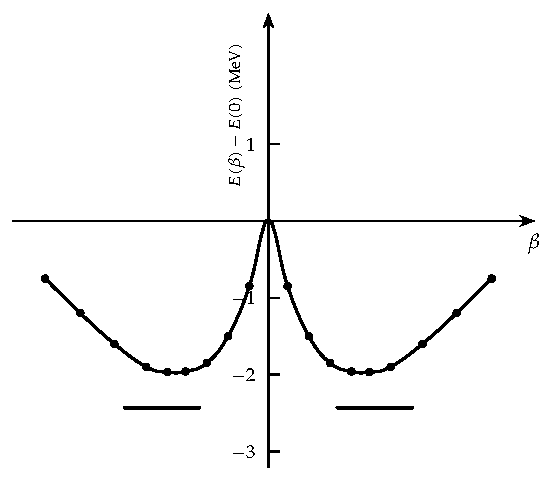
\includegraphics[width=0.6\linewidth]{pictures/7_1}
\par\end{centering}
\centering{}\caption{\label{fig:7_1_Sm152=007ED3=005408=0080FD}作为形变函数的结合能（针对 $\ce{^{152}Sm}$）。极小值之外的横线为自洽计算的解（引自
\cite{DMP66}）。}
\end{figure}

\noindent\textbf{(b) 采用 Skyrme 力的计算}\footnote{利用第 5.6.1.2 节讨论的 Negele 力也进行了类似的计算\cite{NR77}。}。我们在第
5.6.2 节中看到，带有密度依赖 Skyrme 力的 HF 理论能够重现球形核的基态性质。因此它们也被应用于形变情况\cite{Va73}。正如第
7.4 节所讨论的，没有先验的理由对$\Gamma$和$\Delta$的计算采用相同的力。因此，第一步是使用纯配对力 (4.140)
来计算$\Delta$。在时间反演不变的情况下，我们再次发现（如同在对-四极模型中）正则基与$h$为对角矩阵的 HF 基一致。因此，在迭代的每一步中对角化$h$就足够了。与普通
HF 计算唯一的区别在于，在计算密度$\rho,\tau,\boldsymbol{J}$时，我们必须考虑配对能和占据几率$v^{2}_{k}$。代替式
(5.84)，例如我们得到：

\begin{equation}
\rho(\boldsymbol{r})=\sum^{\infty}_{ist}v^{2}_{i}|\varphi_{i}(\boldsymbol{r},s,t)|^{2},\label{eq:skyrme_density_with_pairing}
\end{equation}

其中

\begin{equation}
v^{2}_{i}=\frac{1}{2}\left(1-\frac{\epsilon_{i}-\lambda}{\sqrt{(\epsilon_{i}-\lambda)^{2}+\Delta^{2}}}\right).\label{eq:vi2_skyrme_bcs}
\end{equation}

在此$\lambda$同样由粒子数条件确定。原则上，$\Delta$应当由能隙方程 (6.60) 确定。Vautherin 采取了相反的途径，采用从实验中选取的固定能隙$\Delta$，并利用式
(6.60) 计算了相应的力常数。与球形核 HF 计算的巨大差异在于，在形变核中微分方程 (5.100) 在径向坐标$r$与角度$\theta,\phi$之间不再是可分离的。它现在是一个偏微分方程。Vautherin
通过在各向异性谐振子基中进行对角化求解了该方程。只有矩阵元是在坐标空间中通过高斯积分计算的。轴对称性允许将其分解为具有良好量子数$\Omega$的子空间。尽管如此，这些计算仍然需要巨大的计算工作量\footnote{关于坐标空间中形变 HF 方程的求解，参见 \cite{HN77}。}。

计算结果显示出与实验结合能和半径令人满意的符合。特别地，人们能够重现形变重核测得的四极矩和十六极矩\cite{FQV73}。

\noindent\textbf{(c) 完全 HFB 计算}。正如我们在第 6 章中所见，配对关联不仅取决于有效配对力的性质，还取决于单粒子能级密度。因此，自洽场和配对场由同一种力导出的完全
HFB 计算，仅在 HF 场产生合理的单粒子谱时才具有物理意义。正如第 5 章所讨论的，进行这项任务需要密度依赖的有效力。另一方面，由于现有版本的
Skyrme 力的$\delta$-力性质，它们不适用于完全的 HFB 计算。因此，Gogny \cite{Go73,Go75b,DGG75,DG80}
引入了一种带有有限力程部分的新型密度依赖相互作用（参见第 4.4.4 节）。这种力的高斯形式允许在谐振子基中快速计算矩阵元\cite{Go75a}。

在推导 HFB 方程时，迄今为止我们尚未采用密度依赖力。仿照第 5.6 节，在此时我们必须将能量计算为密度$\rho$和$\kappa$的泛函{[}我们使用式
(E.19) 中定义的约定$\mathrm{Tr}_{1}$和$\mathrm{Tr}_{2}${]}：

\begin{equation}
E'(\rho,\kappa)=\langle\Phi|T+V(\rho)-\lambda\hat{N}|\Phi\rangle=\mathrm{Tr}\,(t-\lambda)\rho+\frac{1}{2}\mathrm{Tr}_{1}\mathrm{Tr}_{1}\rho\bar{v}\rho+\frac{1}{4}\mathrm{Tr}_{2}\mathrm{Tr}_{2}\kappa^{*}\bar{v}\kappa,\label{eq:energy_functional_hfb_density_dep}
\end{equation}

并从变分原理导出 HFB 方程。这通过使用超矩阵$\mathcal{R}$ (7.27) 最容易实现。我们将$(i<k)$的$\rho_{ii},\rho_{ik},\rho^{*}_{ik},\kappa_{ik},\kappa^{*}_{ik}$作为独立变量，并通过
Lagrange 参数矩阵施加关系 (7.28) 作为附加条件（该过程也可以用来推导第 5 章中的普通 HF 方程）：

\begin{equation}
\delta\left(E'(\rho,\kappa)-\mathrm{Tr}(\Lambda(\mathcal{R}^{2}-\mathcal{R}))\right)=0.\label{eq:variational_principle_lagrange_R}
\end{equation}

我们求得：

\begin{equation}
\delta E'=\mathrm{Tr}(\mathcal{H}\cdot\delta\mathcal{R})\label{eq:delta_E_prime}
\end{equation}

其中

\begin{equation}
\delta\mathcal{R}=\begin{pmatrix}\delta\rho & \delta\kappa\\
-\delta\kappa^{*} & -\delta\rho^{*}
\end{pmatrix},\qquad\mathcal{H}=\begin{pmatrix}h & \Delta\\
-\Delta^{*} & -h^{*}
\end{pmatrix}\label{eq:delta_R_supermatrix}
\end{equation}

且

\begin{equation}
h_{ik}=\frac{\delta E'}{\delta\rho_{ki}},\qquad\Delta_{ik}=\frac{\delta E'}{\delta\kappa^{*}_{ik}},\label{eq:hik_deltaik_derivatives}
\end{equation}

在与密度无关力的情况下与式 (7.41) 一致。从式 (7.76) 得到：

\begin{equation}
\mathrm{Tr}((\mathcal{H}-\Lambda\mathcal{R}-\mathcal{R}\Lambda+\Lambda)\delta\mathcal{R})=0.\label{eq:tr_lambda_R}
\end{equation}

由于$\delta\mathcal{R}$是独立变分，这等价于：

\begin{equation}
\mathcal{H}=\Lambda\mathcal{R}+\mathcal{R}\Lambda-\Lambda.\label{eq:H_lambda_R_relation}
\end{equation}

通过条件$\mathcal{R}^{2}=\mathcal{R}$消去$\Lambda$，结果为：

\begin{equation}
[\mathcal{H},\mathcal{R}]=0.\label{eq:H_R_commutator_zero}
\end{equation}

这正是式 (7.43)。它等价于式 (7.36)，并且可以按照求解 HFB 方程 (7.42) 的相同方法求解。然而，在相互作用$v(1,2)$依赖于$\rho$的情况下，我们得到对自洽场$\Gamma$有贡献的额外项。从式
(7.75) 和 (7.79) 可以看出，它们具有如下形式：

\begin{equation}
\frac{1}{4}\frac{\partial}{\partial\rho_{ki}}\mathrm{Tr}_{2}\mathrm{Tr}_{2}(\kappa^{*}\bar{v}[\rho]\kappa).\label{eq:rearrangement_term_pairing}
\end{equation}

通过以合适的方式调节力参数（表 4.4），Gogny 能够重现球形核以及形变核的性质。特别地，他得到了正确的形变与能隙参数（参见表
7.1）。

\begin{table}[H]
\begin{centering}
\caption{\label{tab:7_1_=007ED3=005408=0080FD=007535=008377=0056DB=006781=0077E9=0080FD=009699=006BD4=008F83}结合能
$E$、电荷四极矩 $Q$ 以及质子和中子的能隙参数 $\Delta$ 的实验值与计算值比较（引自 \cite{Go75b}）}
\par\end{centering}
\centering{}%
\begin{tabular}{ccccccccc}
\hline 
核素 & $E_{\text{HFB}}$ {[} & $E_{\text{EXP}}$ {[} & $Q_{\text{HFB}}$ {[} & $Q_{\text{EXP}}$ {[} & $\Delta_{p,\text{HFB}}$ {[} & $\Delta_{p,\text{EXP}}$ {[} & $\Delta_{n,\text{HFB}}$ {[} & $\Delta_{n,\text{EXP}}$ {[}\tabularnewline
\hline 
$\ce{^{150}Sm}$ & 1235.8 & 1239.3 & 383 & 367 & 1.24 & 1.43 & 1.13 & 1.13\tabularnewline
$\ce{^{152}Sm}$ & 1249.0 & 1253.1 & 572 & 590 & 1.14 & 1.08 & 1.09 & 1.24\tabularnewline
$\ce{^{166}Er}$ & 1348.1 & 1351.6 & 770 & 770 & 1.10 & 0.97 & 1.02 & 1.00\tabularnewline
$\ce{^{184}W}$ & 1468.2 & 1472.9 & 631 & 627 & 0.90 & 0.86 & 0.86 & 0.73\tabularnewline
\hline 
\end{tabular}
\end{table}

结合能仍应当针对转动对称性和粒子数破缺所引起的赝贡献进行修正（参见第 11 章）。这些修正可以达到 5 MeV 的数量级\cite{FQV73}。

总结这些结果，我们发现带有密度依赖力的 HFB 理论能够在元素周期表的整个范围内重现球形核与形变核的所有基本基态性质。在下一节中，我们将看到如何将该理论推广到裂变过程能量面的微观计算。

\section{约束Hartree-Fock理论\label{sec:=007EA6=00675FHartree-Fock=007406=008BBA}}

无约束的 HF 和 HFB 计算仅给出能量面上的一个点，即局部极小值。我们通常也对能量面上的其它点感兴趣：我们可以施加某些附加条件，并寻求能量在由它们定义的超曲面上的极小值。有时我们希望将能量面计算为一个（或若干个）集体参数$q$的函数，例如四极或十六极形变。正如我们在第
1 章中所看到的，这是导出集体 Hamilton 量（用于描述集体振动或裂变过程）的第一步。我们将在第 10 章结合生成坐标法更详细地讨论这一点。

在所有这些情况下，我们都对在某个单粒子算符$\hat{Q}$具有固定期望值的约束下使总能量极小化的波函数$|\Phi(q)\rangle$感兴趣：

\begin{equation}
q=\langle\Phi|\hat{Q}|\Phi\rangle.\label{eq:constraint_expectation_q}
\end{equation}

求解该问题的最简单方法是将条件 (7.84) 带有 Lagrange 乘符$\lambda$加到 Hamilton 量$H$中，并求下式的极小值：

\begin{equation}
\langle H'\rangle=\langle H\rangle-\lambda\langle\hat{Q}\rangle.\label{eq:linear_constraint_H_prime}
\end{equation}

在该问题求解之后，$\lambda$由条件 (7.84) 确定。该方法也称为线性约束变分。它对应于考察处于合适地使其发生形变的外场$\hat{Q}$中的多体体系。

该方法已经应用于 BCS 理论（第 6.3.2 节）中，以获得具有粒子数正确期望值的波函数。与式 (6.41) 类似，我们发现 Lagrange
乘符$\lambda$是能量$E=\langle\Phi|H|\Phi\rangle$对$q$的导数：

\begin{equation}
\lambda=\frac{\mathrm{d}E}{\mathrm{d}q}.\label{eq:lambda_dE_dq}
\end{equation}

正如我们从图 7.2 所看到的，线性约束的方法意味着我们必须在点$q=q_{0}$处作能量面$E(q)$的切线，并将该切线作为旋转了角度$\alpha$（其中$\tan\alpha=\lambda$）的新坐标系的$x$轴。新坐标系中的$y$轴对应于$\langle H'\rangle$。对$\langle H'\rangle$进行无约束变分给出了旋转坐标系中能量面的极值。

显然，只要函数$E(q)$具有正的二阶导数，该过程就可以有效工作。在曲线向下凹的情况下——例如在裂变路径上的鞍点附近或在回弯区（图
3.4）——该方法将不再有效。在这些情况下，旋转坐标系中的能量在点$q_{1}$处具有极大值，它永远不会是 HF 方程的稳定解。

\begin{figure}[H]
\begin{centering}
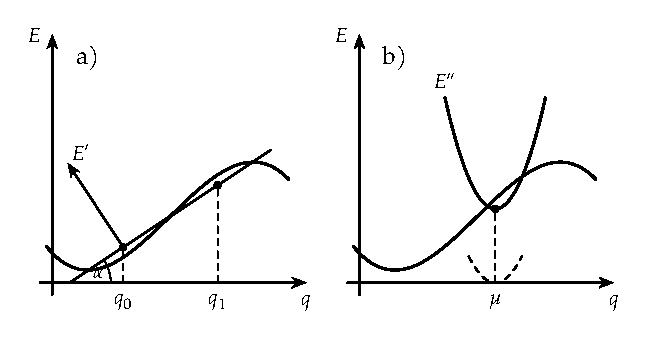
\includegraphics[width=0.7\linewidth]{pictures/7_2}
\par\end{centering}
\centering{}\caption{\label{fig:7_2_=0080FD=0091CF=009762=007EA6=00675F=00793A=00610F=0056FE}示意性能量面，展示了线性约束（a）与二次约束（b）的方法。}
\end{figure}

我们还认识到，在拐点附近总是存在若干个具有平行切线的点（即具有相同的$\lambda$，但具有不同的$q$值），也就是说，$q$不再是
Lagrange 参数的单值函数（参见图 3.6）。

存在若干种避免该问题并寻找能量面上此类点的波函数的方法：

(i) 梯度法（如第 7.3 节所讨论）允许我们沿着垂直于对$\hat{Q}$的梯度的最速下降线前进。因此，对于每个$q$值，我们都能找到相应的能量极小值。

(ii) 二次约束法\cite{GLW70,FQK73}采用对函数

\begin{equation}
E''=\langle H\rangle+\frac{1}{2}C(\langle\hat{Q}\rangle-\mu)^{2}\label{eq:quadratic_constraint_function}
\end{equation}

的无约束变分。如图 7.2b 所示，这里我们在能量面上添加了一条对称轴为$q=\mu$的抛物线。它产生了一个在$\mu$附近具有极值的新曲面$E''$。如果其宽度充分小（$C>|\mathrm{d}^{2}E/\mathrm{d}q^{2}|$），这始终是一个真正的极小值。$E''$的变分给出：

\begin{equation}
\delta\langle H\rangle-C(\mu-\langle\hat{Q}\rangle)\delta\langle\hat{Q}\rangle=0.\label{eq:variation_E_double_prime}
\end{equation}

这意味着二次约束等价于具有$\lambda=C(\mu-\langle\hat{Q}\rangle)$的线性约束。在两种情况下，我们得到相同的能量面。对于作为$\langle\hat{Q}\rangle$的函数的任何约束，这都是正确的。采用二次约束，$\lambda$的有效值在迭代过程中自动改变。

(iii) 第三种方法\cite{BW71}使用线性约束，但在迭代的每一步中改变$\lambda$的值，使得条件 (7.84)
得到满足。该方法应用于带有粒子数约束的 BCS 计算中。然而，它需要在每一步进行额外的迭代。

约束 Hartree-Fock 理论（CHF）已被用于计算原子核在基态附近的能量面\cite{BKS67,CLF73,CS73,FQK73,GG78}以及裂变过程\cite{FQV74,KCS74,BFV74}。

在后一种情况下，通常必须面对应当使用何种约束算符$\hat{Q}$的问题。容易证明，通过使用合适的约束算符$\hat{Q}_{\Phi}$进行
CHF 计算，我们可以找到任何乘积波函数$|\Phi\rangle$。我们只需使用双准粒子部分$Q^{20}$被定义为$H^{20}$的倍数的算符。随后我们得到：

\begin{equation}
H^{20}-\lambda Q^{20}=0,\label{eq:chf_q20_condition}
\end{equation}

也就是说，$|\Phi\rangle$作为相应 CHF 方程的解。当然，这对于计算$|\Phi\rangle$没有太大的实用价值，但它表明存在种类繁多的约束算符，它们产生相同的波函数，仅在它们的$Q^{11}$-矩阵元上有所不同。

\begin{figure}[H]
\begin{centering}
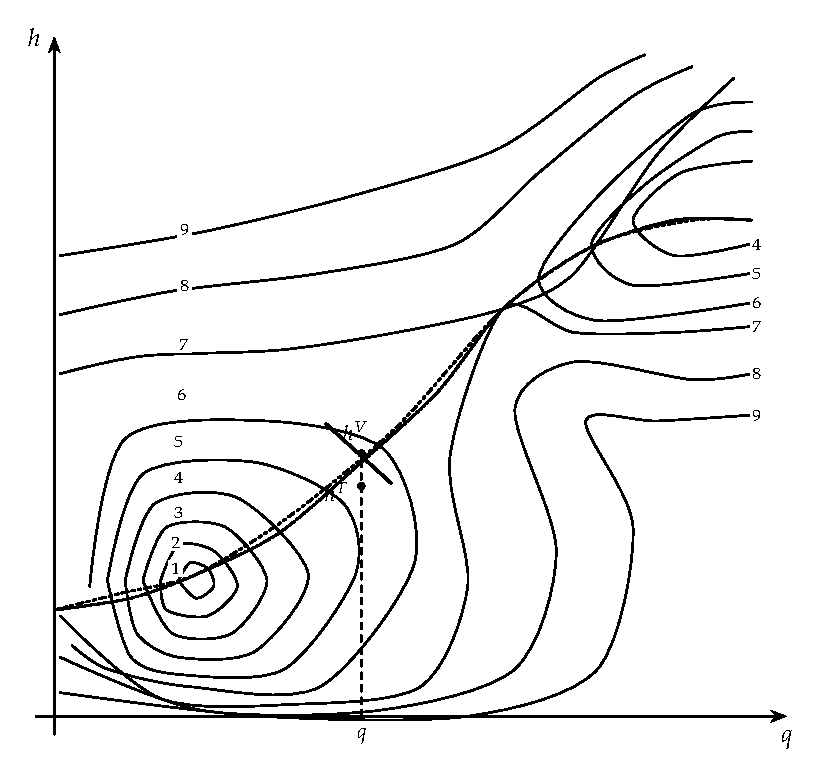
\includegraphics[width=0.65\linewidth]{pictures/7_3}
\par\end{centering}
\centering{}\caption{\label{fig:7_3_qh=0080FD=0091CF=009762=0088C2=0053D8=008C37}$(q,h)$
平面内的能量面示例，表明仅对 $q$ 加约束并不能精确跟踪裂变谷（引自 \cite{FQK73}）。}
\end{figure}

另一方面，对一种形变的约束（例如四极形变$q=\langle\Phi|Q_{20}|\Phi\rangle$）并不意味着另一种形变（例如十六极形变$h=\langle\Phi|Q_{40}|\Phi\rangle$）保持不变。这在图
7.3 中示意性地给出。只要我们对$q$使用约束，我们就沿着线$h^{1}(q)=\langle\Phi(q)|Q_{40}|\Phi(q)\rangle$行进。它连接了每个等势面上的垂直切点，因为对于恒定的$q$，$E$必须对所有其它自由度达到极小，这意味着特别是$\mathrm{d}E/\mathrm{d}h|_{q=\text{const}}=0$。这条线$h^{1}(q)$通常与裂变谷底不同，后者对应于最速下降线$h^{0}(q)$。两条线都穿过能量面的驻点，例如基态极小值或鞍点。如果裂变谷平行于$q$轴，这两条线非常接近；但如果裂变谷平行于$h$轴，它们可能会发生相当剧烈的偏离。尽管如此，与液滴模型和
Strutinsky 式计算（参见第 2.9 节）相比，我们认识到 CHF 计算的巨大优势：在 CHF 计算中，我们只需追踪单参数曲线，就能获得在许多情况下与裂变谷底非常接近的波函数，而在其它方法中我们必须计算多维能量面。

在 CHF 计算中，我们当然应该优化约束算符的选择。在第 10 章中，我们将研究实现这一目标的方法。

\begin{figure}[H]
\begin{centering}
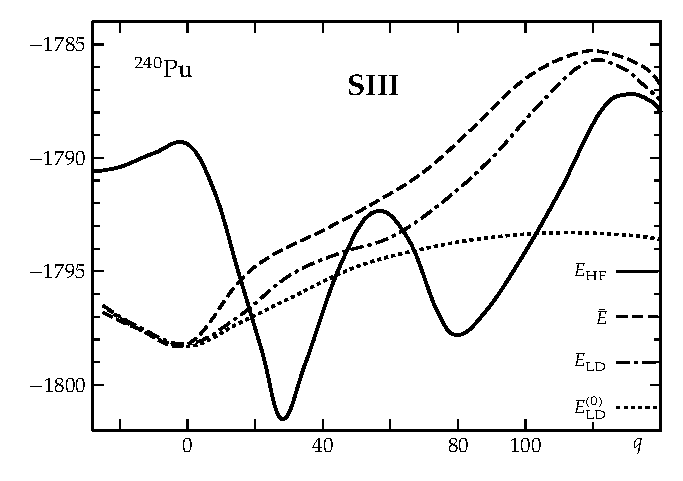
\includegraphics[width=0.65\linewidth]{pictures/7_4}
\par\end{centering}
\centering{}\caption{\label{fig:7_4_Pu240=005F62=0053D8=0080FD=0066F2=007EBF}利用 Skyrme
III 相互作用作为质量四极矩 $q$ 的函数计算出的 $\ce{^{240}Pu}$ 形变能曲线。详细说明见正文（引自 \cite{BQ75a}）。}
\end{figure}

图 7.4 展示了利用带有质量四极矩$q$约束的 Skyrme 力计算得到的原子核$\ce{^{240}Pu}$的形变能（实线\cite{FQV74}）。对关联通过简单的对力来考虑，其常数$G$选为与核表面积成正比。该计算重现了基态极小值和第二极小值。势垒的高度在定量上与实验数据不符，但我们必须记住，在计算中保持了轴对称性和空间反射宇称，而有迹象表明实际的裂变路径在内鞍点破坏了轴对称性，在外界鞍点破坏了空间反射宇称。

为了将这些结果与液滴模型计算进行比较，计算了 Strutinski 平均的 HF 能量（虚线）并显示在图 7.4 中。它显示出微小的起伏波动。然而，这些起伏并不是由壳效应引起的，它们也存在于对应于相同形变$q$和$h$的液滴能量中（点划线），因为该曲线与侧谷相交。裂变谷底的液滴能量（点线）是非常平滑的。

图 7.5 显示了同一原子核在不同形变下的质子密度分布。

\begin{figure}[H]
\begin{centering}
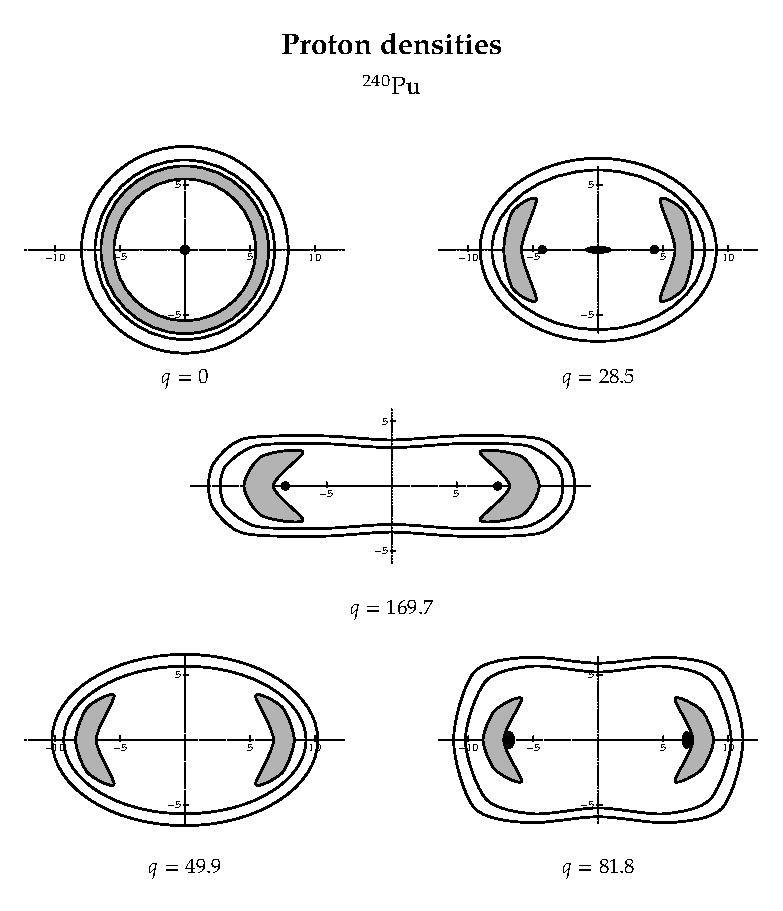
\includegraphics[width=0.7\linewidth]{pictures/7_5}
\par\end{centering}
\centering{}\caption{\label{fig:7_5_Pu240=008D28=005B50=005BC6=005EA6=005206=005E03}$\ce{^{240}Pu}$
在不同形变 $q=\langle Q_{20}\rangle$ 下的质子密度分布（引自 \cite{FQV74}）。}
\end{figure}

若干作者\cite{FS76,BSV76}指出，如果允许波函数$|\Phi\rangle$在空间中扩展得非常远，带有具有无界能谱约束算符（例如当$r\to\infty$时发散的$Q\sim r^{2}Y_{20}$）的此类
CHF 计算可能会给出非常虚假的解。然而，CHF 方法的所有实际应用都是在有限组态空间中进行的，这确保了波函数$|\Phi\rangle$定域在原子核的区域内。

因此，在组态空间的选择上，我们受到来自两方面的限制：为了获得结合能的收敛，通常需要大的组态空间；但另一方面，我们不应该能够表象上述的虚假解。看来迄今为止进行的
CHF 计算都保持在这些限制之内。

保持核波函数定域的另一种可能途径是引入第二个约束\cite{GL77}：

\begin{equation}
\hat{H}'=\hat{H}-\lambda\hat{Q}+\mu\hat{Q}^{2}.\label{eq:second_constraint_operator}
\end{equation}

Lagrange 参数$\mu$将允许我们改变波函数中的$\langle\Delta\hat{Q}^{2}\rangle$涨落。

\section{转动系下的HFB理论\label{sec:=008F6C=0052A8=007CFB=004E0B=007684HFB=007406=008BBA}}

在第 3 章中，我们在纯单粒子壳模型的框架内讨论了 cranking 模型。它为我们提供了微观计算转动惯量的可能性。显而易见如何将该理论推广到自洽多体体系：我们必须在角动量算符$J_{x}$具有确定期望值的附加条件下，对多体
Hamilton 量$H$的期望值进行变分。这给出了方程（亦参见第 11.4 节）：

\begin{equation}
\delta\langle\Phi|H-\omega J_{x}|\Phi\rangle=0.\label{eq:cranking_variation_scc}
\end{equation}

cranking 频率$\omega$依赖于角动量$I$，并由下式确定：

\begin{equation}
\langle\Phi_{\omega}|J_{x}|\Phi_{\omega}\rangle=\sqrt{I(I+1)}.\label{eq:cranking_frequency_condition}
\end{equation}

在第 11 章中我们将看到，该问题的解$|\Phi_{\omega(I)}\rangle$必须被理解为内禀波函数，在实验室坐标系中通过投影到好的角动量上可以从中获得$\boldsymbol{J}^{2}$的本征函数。

在 HFB 理论中，我们将变分函数的集合$|\Phi\rangle$限制为 HFB 类型的广义乘积函数，这样我们便面对一个带有约束的
HFB 问题。类似于单粒子情况下的 cranking 模型，该方法被称为自洽 cranking 模型（self-consistent
cranking model, SCC）。在上一节中，我们已经非常详细地讨论了约束 HF 方法的问题。在回弯区（参见第 3 章以及
\cite{CMR75}），式 (7.91) 的解对应于在恒定$\omega$下能量面上的鞍点。因此，我们必须应用梯度法或二次约束以在回折分支上获得解。

与迄今为止所讨论的 HFB 理论的应用不同，波函数$|\Phi\rangle$的时间反演对称性被算符$\omega J_{x}$破坏。因此，我们无法先验地知道正则基中的共轭态，从而必须在转动系中求解完全的
HFB 问题\cite{RBM70}，即：

\begin{equation}
\begin{pmatrix}h-\omega j_{x} & \Delta\\
-\Delta^{*} & -h^{*}+\omega j^{*}_{x}
\end{pmatrix}\begin{pmatrix}U_{k}\\
V_{k}
\end{pmatrix}=\begin{pmatrix}U_{k}\\
V_{k}
\end{pmatrix}E_{k}.\label{eq:cranking_hfb_equation}
\end{equation}

利用被 cranking Hamilton 量所保持的对称性$\mathrm{e}^{\mathrm{i}\pi j_{x}}$，矩阵$\rho,\kappa,\Gamma$以及$\Delta$具有形式
(7.67)。由于时间反演对称性$T$被破坏，代替式 (7.69)，我们有：

\begin{equation}
\rho_{2}\ne\rho^{*}_{1};\qquad\Gamma_{2}\ne\Gamma^{*}_{1};\qquad D_{2}\ne D^{*}_{1};\qquad\kappa^{\dagger}_{1}\ne\kappa_{1};\qquad\Delta^{\dagger}_{1}\ne\Delta_{1}.\label{eq:time_reversal_broken_relations}
\end{equation}

因此，密度和势具有时间偶部分和时间奇部分，例如：

\begin{equation}
\rho^{(+)}=\rho_{1}+\rho^{*}_{2};\qquad\rho^{(-)}=\rho_{1}-\rho^{*}_{2}.\label{eq:rho_time_even_odd}
\end{equation}

在$\omega=0$时二重简并的准粒子能量$E_{k}$（参见第 2.8 节），在有限的 cranking 频率下发生分裂（图
7.8d），并且不再由公式 (7.51) 给出。然而，根据 Bloch-Messiah 定理 (7.7)，存在一个正则基，可以通过对角化密度$\rho$找到。正如我们从式
(7.50) 可以看出的，在此基下的占据几率$v^{2}_{k}$由下式给出：

\begin{equation}
v^{2}_{k}=\frac{1}{2}\left[1-\frac{\epsilon_{k}-\omega j_{x_{k}}}{\sqrt{(\epsilon_{k}-\omega j_{x_{k}})^{2}+\Delta^{2}_{k\bar{k}}}}\right],\label{eq:vk2_cranking_canonical}
\end{equation}

其中$\epsilon_{k}=\frac{1}{2}(h_{kk}+h_{\bar{k}\bar{k}})$且$j_{x_{k}}=\frac{1}{2}(j_{x_{kk}}+j_{x_{\bar{k}\bar{k}}})$。

这表明在正则基下的对角矩阵元$h_{kk},j_{x_{kk}},h_{\bar{k}\bar{k}},j_{x_{\bar{k}\bar{k}}}$以及$\Delta_{k\bar{k}}$是决定占据几率的关键量。矩阵$h,j_{x}$和$\Delta$本身在此基下通常不是对角的。人们还会注意到，具有较大正矩阵元$j_{x_{k}}$的能级比较大负值的能级具有更大的占据几率。

自洽 cranking 模型对于描述高自旋区发现的异常现象非常有用\footnote{最近，cranking 模型用于描述带交叉的有效性已成为讨论的对象 \cite{Ha76,Ha77,MG78,GSF78b,CDS78}。}，这些现象在第
3 章中曾予以讨论。它足够普遍，能够涵盖种类繁多的物理效应。为了说明这一点，我们将讨论原子核$\ce{^{164}Er}$的某些效应，该核在近几年中在实验上得到了非常深入的研究\cite{LCS76,KSM78}。人们已经发现了延伸至相当高自旋值的若干条转动带（参见图
7.6）。

\begin{figure}[H]
\begin{centering}
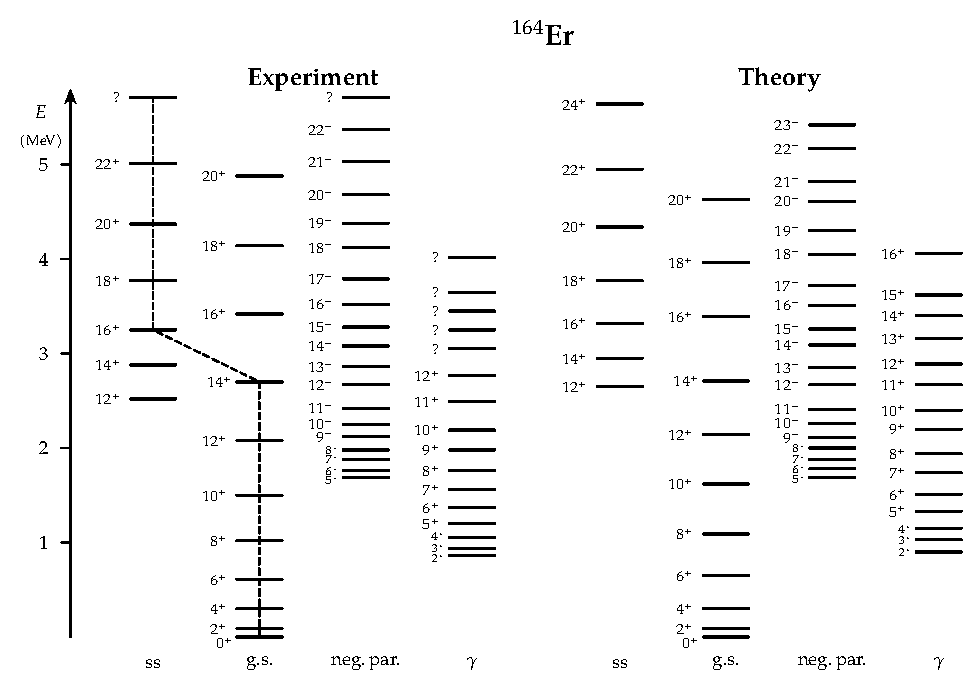
\includegraphics[width=0.7\linewidth]{pictures/7_6}
\par\end{centering}
\centering{}\caption{\label{fig:7_6_Er164=008F6C=0052A8=005E26=0080FD=008C31}$\ce{^{164}Er}$
中的转动带能谱。除基态带（gs）外，还展示了由对准的 $i_{13/2}$ 中子对构成的 Stephens-Simon 带（ss）、负宇称带和
$\gamma$ 带 \cite{KSM78}。Yrast 线（虚线所示）沿着每个 $I$ 值的最低能级。右侧给出了 SCC
方法的理论计算结果 \cite{MSR76,EMR80a,EMR80b}。}
\end{figure}

方程 (7.91) 的变分给出了每个$I$值的最低能量。根据定义，这就是 yrast 线（图 7.6 中的虚线）。正如我们所见，它仅在$I=14$之前跟随基态带。在$I=14$与$I=16$之间，出现了一个带交叉，也就是说，如果我们沿着
yrast 线就会发生回弯（参见图 7.7）。相交叉的带具有带有两个对准的$i_{13/2}$中子的双准粒子带的结构。因此，yrast
线改变了它的性质：它在$I=14$之前跟随基态带，而对于所有$I\geqslant16$的值对应于对准带。在自洽 cranking
模型内沿着 yrast 线的能级计算展现出以下特征：

\begin{figure}[H]
\begin{centering}
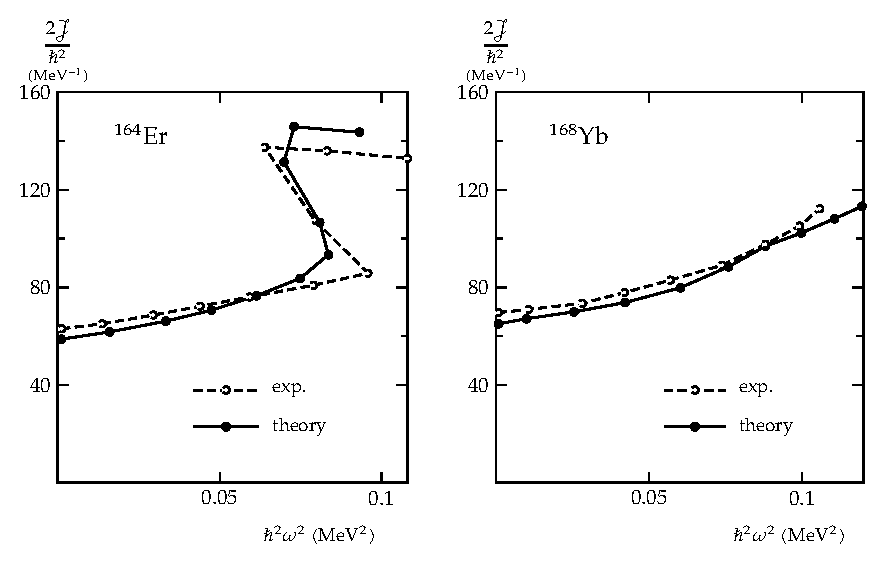
\includegraphics[width=0.7\linewidth]{pictures/7_7}
\par\end{centering}
\centering{}\caption{\label{fig:7_7_Er164_Yb168=0056DE=005F2F=0056FE}原子核 $\ce{^{164}Er}$
和 $\ce{^{168}Yb}$ 的回弯图。虚线代表实验数据，实线为 SCC 理论的计算结果 \cite{MSR76}。转动惯量
$\mathcal{J}$ 和角频率 $\omega$ 的定义见式 (3.3)。}
\end{figure}

\noindent\textbf{(i) 伸展效应（The Stretching Effect）}代表转动过程中核形变可能发生的变化。它由自洽势$\Gamma$所描述，该势依赖于密度，因而依赖于
cranking 频率。图 7.8a 显示了在$\ce{^{164}Er}$的 SCC 计算中发现的有效核形变$\beta$和$\gamma$。在此自旋区域内形变$\beta$的改变相当小。对于许多良好形变的稀土核也是如此。另一方面，$\gamma$-形变增加至$\gamma\sim10^{\circ}$，但这强烈依赖于具体原子核，其它原子核对于$\gamma$-形变可能相当刚硬。

\noindent\textbf{(ii) Coriolis 反配对效应（The Coriolis Antipairing Effect,
CAP）}意味着核内的对关联被 Coriolis 力削弱。在第 6 章中我们看到，对关联主要来源于相反自旋的核子对（Cooper 对），由于它们具有大的空间重叠而感受到强相互作用。由于
Coriolis 力在相反方向作用于两个角动量上（图 7.9），我们应当预期至少会出现部分对准以及相应的配对能$\Delta$随自旋增加而降低。这在计算中得到了证实（图
7.8b），并解释了低自旋值下转动惯量的适度增加。正如磁场中的超导体一样，在某一临界角动量下，我们发现了向正常流体态的相变。这种核
Meissner 效应由 Mottelson 和 Valatin \cite{MV60} 所预言，并在许多计算中（例如 \cite{CV66,RBM70,Wa70a,Ku72,Fr76}）在各不相同的自旋值下被发现。

\begin{figure}[H]
\begin{centering}
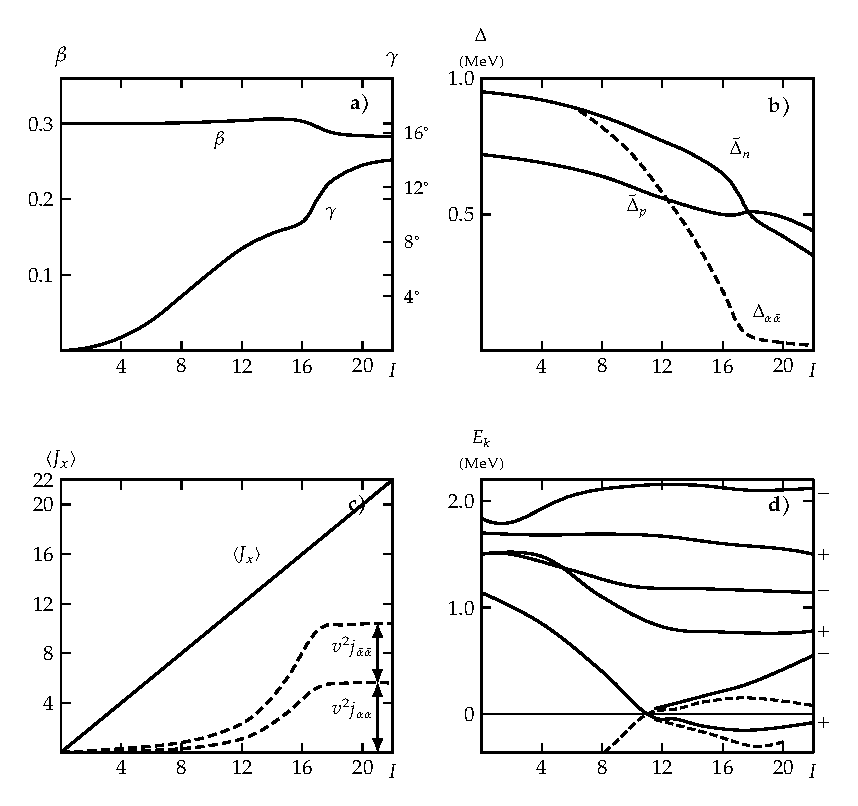
\includegraphics[width=0.7\linewidth]{pictures/7_8}
\par\end{centering}
\centering{}\caption{\label{fig:7_8_Er164=007406=008BBA=0053C2=006570=0053D8=005316}$\ce{^{164}Er}$
计算得到的形变参数（a）、能隙参数（b）、角动量期望值 $J_{x}$（c）以及转动系中的准粒子能量 $E_{k}$（d）随角动量的变化（引自
\cite{MSR76}）。$\beta$ 形变的值归一化为 $I=0$ 时的 0.3。部分（b）显示了质子和中子在正则基下的平均能隙参数
$\tilde{\Delta}_{p}$ 与 $\tilde{\Delta}_{n}$ {[}式 (7.97){]} 以及对准对的能隙参数
$\Delta_{\alpha\bar{\alpha}}$（虚线）。更详细的说明见正文。}
\end{figure}

\begin{figure}[H]
\begin{centering}
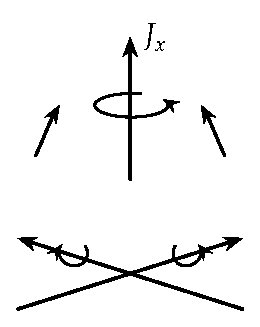
\includegraphics[width=0.45\linewidth]{pictures/7_9}
\par\end{centering}
\centering{}\caption{\label{fig:7_9_CAP=006548=005E94=00793A=00610F=0056FE}Coriolis 反配对效应（CAP）的示意图。}
\end{figure}

回弯现象曾被认为是由这种相变引起的\cite{KS73}。然而，允许一对或几对核子发生解耦过程的更现实计算表明，配对能隙$\Delta$在回弯区域并没有完全消失（图
7.8b，在$I=12$和$I=16$之间）。由于对准过程，它仅仅是减小了。这对应于向具有相应阻塞效应的双准粒子带的转变（参见第
6.3.4 节）。在图 7.8b 中，我们展示了平均能隙：

\begin{equation}
\tilde{\Delta}=\frac{1}{M'}\sum^{M'}_{k>0}\Delta_{k\bar{k}}.\label{eq:average_gap_def}
\end{equation}

（$M'=M/2$是组态空间中$k>0$的能级数。）即使对于在原始基下具有常数配对矩阵元$\Delta$的常数配对力，在正则基下的所有矩阵元$\Delta_{k\bar{k}}$也并不都相等。特别地，对准对的矩阵元$\Delta_{\alpha\bar{\alpha}}$趋向于零（图
7.8b 中的虚线）。这种效应对于仅作用于$I=0$对的纯配对力表现得最为显著（参见第 4.4.7 节）。极高自旋态的现实计算仍有待进行。然而，模型计算和实验数据\cite{BSC75}表明，剩余的对关联仍然存在，有时甚至维持到相当高的自旋值（$I\sim40\text{--}50\hbar$）。

\noindent\textbf{(iii) 对准过程（Alignment Processes）}（Stephens-Simon
效应，\cite{SS72a}；参见第 3.2 节）。由于 HFB 波函数$|\Phi\rangle$是最普遍的单粒子态的乘积（具有相应的占据几率），它们不仅可以代表基态带，还可以代表部分或完全对准的双准粒子带的态。因此，它们是在微观上研究此类解耦过程的合适工具。然而显然，我们必须允许轴对称性的破坏以描述此类对准态，它们是许多不同$\Omega$值的混合（参见第
3.3 节）。这在 cranking 计算中不成问题，因为 Coriolis 项$\omega j_{x}$无论如何都破坏了这种对称性。

对准的程度由两粒子在正则基下的矩阵元$j_{x_{\alpha\alpha}}$和$j_{x_{\bar{\alpha}\bar{\alpha}}}$来量度。图
7.8c 展示了这些数值{[}乘以相应的占据几率 (7.96)，后者事实上非常接近于 1{]}以及$J_{x}$的总期望值。人们注意到，在回弯区，$J_{x}$总增量的大部分以上来自于这一对粒子。其余粒子的贡献减少，这对应于该区域内角频率$\omega$的减小。对于更高的自旋值，对准对的贡献相当稳定在$5.8+4.8\simeq10.6$，而一个完全对准的$i_{13/2}$对将给出$13/2+11/2=12$。

\noindent (iv) 最后，图 7.8d 展示了转动系中的某些准粒子能量 $E_{k}$\}，它们是式 (7.93) 的本征值随角动量的变化。它们不再是二重简并的，而在时间反演不变的情况下是二重简并的。在大角动量下，可能会发生这些能量之一趋于零并变为负值的情况。由于配对势在该区域并未消失，该现象被称为无能隙超导（gapless
superconductivity）\footnote{在金属超导体中也出现类似的现象 \cite{AG61}。}
\cite{GLS67,Gr74,CMR75}。然而，这并不意味着存在更低能量的激发态，因为偶体系中的激发能始终是两个准粒子能量之和。我们看到，对于式
(7.93) 的每个本征值$E_{k}$，我们也有一个本征值$-E_{k}$（虚线）。这些“非物理”本征值之一在回弯区变为正值。然而，我们不被允许选取这个正本征值，因为（正如在第
7.3.2 节中所讨论的）这将对应于向奇粒子数体系波函数的转变。我们还在图 7.8d 中（通过细线）标出了带交叉现象，该现象与回弯区从基态带向双准粒子带的转变相关联。

在稀土区的所有原子核中都发现了类似的特征\footnote{关于 SCC 理论在轻核中的应用，参见 \cite{PM76,NS78,Zi78}。}。然而，在回弯图上存在显著的差异（参见图
7.7），因为此类图对能谱能级间距的微小改变非常敏感。在许多情况下，此类对准过程确实发生而并不伴随回弯现象。正如模型计算\cite{CMR75}所示，是否发生回弯取决于底层的单粒子能级密度以及两个相交叉带之间的剩余相互作用：弱相互作用和低能级密度给出突然对准，因而导致回弯。在其它情况（例如$\ce{^{168}Yb}$）下，我们具有平滑的对准过程而没有回弯（亦参见第
122 页的脚注）。

此类计算最初由慕尼黑小组\cite{BMR73}在有限组态空间中利用对-四极相互作用完成。与此同时，该理论已通过粒子数投影得到了改进\cite{DBM73,FDG76}。正如第
11 章所讨论的，这在对关联经历剧烈改变的区域中似乎是必要的。定量上与实验的符合通过此类计算得到了一定程度的改善，但上面讨论的定性图像没有任何改变。将四极对力包含在内也是如此\cite{WF78a}。

人们还使用了更现实的力，如在有限空间中从 Reid 软芯势导出的$G$-矩阵\cite{GVS76,Go76a}或 Skyrme
类型的相互作用\cite{FMR79}。发现了定性上相似的结果。

在第 7.3.2 节中我们看到，我们不仅可以将 HFB 类型的函数$|\Phi\rangle$用于偶核基态以及沿着 yrast 线的态，还可以用于偶核和奇核中的所有类型的准粒子态。因此，在
SCC 方法中，我们还可以描述奇核中的转动带以及偶核中的一般双准粒子带。特别地，我们可以研究所有类型的对准过程。

第 11 章中对 cranking 模型更基本的推导表明，我们应当使用附加条件：

\begin{equation}
\langle J_{x}\rangle=\sqrt{I(I+1)-\langle J^{2}_{z}\rangle}\label{eq:cranking_condition_exact_projection}
\end{equation}

代替式 (7.92)。对于良好近似下轴对称的偶核基态带，$\langle J^{2}_{z}\rangle$相当小。在这些情况下，式
(7.98) 等价于式 (7.92)。利用这一附加条件计算了奇核中严重受扰动的转动带\cite{RMB74,FDB77}，并发现与实验能谱很好地符合（图
3.11）。特别地，在该模型中无需对 Coriolis 相互作用进行任何衰减因子修正\cite{RM74,Ri77}。

图 7.6 给出了具有负宇称的双准粒子带的例子。在这里一个中子位于$i_{13/2}$壳层，另一个中子位于负宇称壳层。我们再次观察到一个$i_{13/2}$中子的对准过程，这引起该带较低能级具有小的能级间距。由于宇称选择定则，相应的波函数自动与基态正交。这在引起回弯现象的所谓“第二”带的计算中是不同的。它是一个激发带，在回弯点处其特征从对准的双准粒子带转变为基态带。该带具有与
yrast 带相同的对称性。因此，我们必须施加额外的约束，即其波函数与 yrast 带的相应波函数正交\cite{EMR80a}。

图 7.6 还展示了一条$\gamma$-带。正如我们将在下一章看到的，此类集体振动无法由纯乘积波函数来描述。然而，这并不意味着建立在此类振动上的转动带不能用
cranking 模型进行研究。我们只需对$|\Phi\rangle$采用更复杂结构的波函数（例如下一章讨论的 TDA 或 RPA
波函数；\cite{Ho68,CMR75,Ma77a,ERM78,ERM80b}）。

让我们以如下总结性评述结束本章：HFB 理论是一种在推广的静态单粒子图像中包含尽可能多的关联的方法。因此，它定义了两个自洽确定的场{[}即序参量（参见第
11 章）{]}：用于$ph$-关联的平均势$\Gamma$，以及用于$pp$-关联的配对势$\Delta$。在这一理论框架内，我们能够重现球形核与形变核的基态性质。它还可以用于描述具有广义乘积类型波函数的激发态，例如纯准粒子激发或良好形变核中的转动态。在后一种情况下，必须对平均角动量施加约束。然而，我们应该记住，形变波函数必须被理解为内禀波函数，在实验室坐标系中通过投影到角动量本征态上可以从中获得波函数（参见第
11.4 节）。

此外，HFB 理论可用于为处理进一步关联的更复杂方法提供最优基。这将在后续章节中进行。
